\documentclass[11pt]{article}

\usepackage{amsmath}
\usepackage{amssymb}
\usepackage{amsthm}
\usepackage{physics}
\usepackage[margin=1in]{geometry}
\usepackage{enumitem}
\usepackage{tikz}
\usetikzlibrary{arrows.meta,backgrounds}

\newcommand{\Vsp}{(V, \oplus, \odot)}
\newcommand{\dual}{V^{*}}
\newcommand{\linto}{\overset{\sim}{\longrightarrow}}

\title{Chapter 2 --- Vector Spaces\\ \large Exercises}
\author{From Differential Geometry to General Relativity --- Study Companion}
\date{}

\begin{document}
\maketitle

\noindent This file is self-contained: everything needed to state and solve
the problems below is introduced inline, in the book's own notation, no
outside reference is required. Problems are organized by topic, following
the logical order in which the chapter builds up the theory; within each
topic, a short motivating question comes first (why this topic exists at
all), then notation, then problems (easy $\to$ hard), then solutions (only
for problems solved so far).

% =============================================================================
\section{Maps and Bijections}
% =============================================================================

\subsection*{Motivation}

\paragraph{Why maps at all.}
The same physical situation can be described in many ways: Celsius or Fahrenheit, Cartesian or polar coordinates, the basis of one observer or another. Every such change of description is a \emph{map}, a rule that turns each description in one list into a description in another. Two questions decide whether a change of description is trustworthy. First, does it lose information, i.e.\ can two different situations end up with the same new description? Second, is anything left out, i.e.\ does every new description correspond to some old one? A map that answers ``no'' to the first and ``yes'' to the second is called a \emph{bijection}, and only bijections can be undone.

\paragraph{Examples.}
The conversion $T_F=\tfrac95T_C+32$ from Celsius to Fahrenheit can be undone, so no information is lost. The rule $x\mapsto|x|$ cannot be undone, since $+3$ and $-3$ both go to $3$: the sign is lost. Passing from polar coordinates $(r,\theta)$ to Cartesian $(x,y)$ loses information at $r=0$ (every $\theta$ gives the same point) and if $\theta$ is allowed to range over more than one full turn; this is why coordinate systems on curved spaces later come with restricted domains.

\paragraph{Composition.}
Suppose you know how to convert $x\to y$, and separately $y\to z$. Is there any ambiguity in the composite conversion $x\to z$, depending on whether you think of it as ``first do $x\to y$, then the result to $z$'' or ``first combine the two later steps, then apply the whole thing to $x$''? And if each step is invertible, is the composite automatically invertible, and in what order do you undo the steps? These questions look almost too obvious to ask, yet the machinery of changing coordinates and bases later in this chapter rests on the answers being ``no ambiguity'' and ``yes, automatically invertible, by undoing the steps in reverse order''.

\subsection*{Notation and Definitions}

\subsubsection*{Maps}
Let $\mathcal M,\mathcal N$ be sets. A \emph{map} $\phi:\mathcal M\to\mathcal N$, written $p\mapsto\phi(p)$, assigns to every $p\in\mathcal M$ exactly one element $\phi(p)\in\mathcal N$. The set $\mathcal M$ is the \emph{domain} and $\mathcal N$ the \emph{codomain}. Both are part of the definition of the map: the formula $p\mapsto p^2$ defines different maps on $\mathbb R\to\mathbb R$ and on $\mathbb R_{\ge0}\to\mathbb R_{\ge0}$.

\subsubsection*{Injective, surjective, bijective}
\begin{itemize}
  \item $\phi$ is \emph{injective} (``no two points are merged'') if $\forall p_1,p_2\in\mathcal M,\ \phi(p_1)=\phi(p_2)\iff p_1=p_2$. (The direction $\Leftarrow$ holds for every map; the content is $\Rightarrow$.)
  \item $\phi$ is \emph{surjective} (``nothing in $\mathcal N$ is missed'') if $\forall n\in\mathcal N,\ \exists p\in\mathcal M:\phi(p)=n$.
  \item $\phi$ is \emph{bijective} if it is both injective and surjective; it then has an inverse map $\phi^{-1}:\mathcal N\to\mathcal M$ with $\phi^{-1}\circ\phi=\mathrm{id}_{\mathcal M}$ and $\phi\circ\phi^{-1}=\mathrm{id}_{\mathcal N}$, where $\mathrm{id}_{\mathcal M}(p):=p$ denotes the \emph{identity map} on $\mathcal M$ (it sends every element of $\mathcal M$ to itself) and $\circ$ denotes composition, $(\varphi\circ\phi)(p):=\varphi(\phi(p))$.
\end{itemize}
Why is bijectivity exactly the condition for an inverse? To define $\phi^{-1}(n)$ we need \emph{some} $p$ with $\phi(p)=n$ (surjectivity) and it must be \emph{only one} such $p$, otherwise $\phi^{-1}(n)$ would not be a single element (injectivity).

\subsubsection*{Composition is associative}
For any composable maps $h:\mathcal A\to\mathcal B$, $g:\mathcal B\to\mathcal C$, $f:\mathcal C\to\mathcal D$,
\[
(f\circ g)\circ h = f\circ(g\circ h).
\]
Indeed both sides are maps $\mathcal A\to\mathcal D$, and for every $a\in\mathcal A$, $[(f\circ g)\circ h](a) = (f\circ g)(h(a)) = f(g(h(a)))$ while $[f\circ(g\circ h)](a) = f((g\circ h)(a)) = f(g(h(a)))$: the same value. Two maps with the same domain and codomain agreeing at every point are equal, so the two bracketings define the same map. This is a structural fact about $\circ$ itself, true for any maps (not only bijections), so composition of three or more maps can be written without parentheses, $f\circ g\circ h$.

\subsubsection*{Example}
Let $\phi:\mathbb R\to\mathbb R$, $\phi(p):=2p+1$. It is injective ($2p_1+1=2p_2+1\Rightarrow p_1=p_2$) and surjective (given $n$, take $p=(n-1)/2$), hence bijective, with $\phi^{-1}(n)=(n-1)/2$. Check: $\phi^{-1}(\phi(p))=\big((2p+1)-1\big)/2=p$.

\subsection*{Common pitfalls and limitations}

\begin{itemize}
  \item \textbf{Bijectivity depends on domain and codomain, not just the formula.} The same rule can be non-injective or non-surjective on one choice of sets and bijective on another.
  \item \textbf{Composition is not commutative.} In general $\varphi\circ\phi\neq\phi\circ\varphi$ (and often only one of the two even makes sense). Only associativity is available.
  \item \textbf{Order reverses when inverting a composite.} To undo ``first $\phi$, then $\varphi$'' you must undo $\varphi$ first, then $\phi$.
  \item \textbf{$\phi^{-1}$ is not $1/\phi$.} The inverse map is unrelated to the reciprocal of the values.
  \item \textbf{One-sided inverses are not enough.} A map with $\phi^{-1}\circ\phi=\mathrm{id}$ only (a left inverse) need not be surjective; an inverse in the sense above requires both identities.
\end{itemize}

\subsection*{Problems}

\begin{enumerate}[label=\textbf{2.\arabic*}, leftmargin=2.2cm]

\item \label{prob:maps}
Consider the map $\phi : \mathbb{R} \longrightarrow \mathbb{R}$, $\phi(p) := p^2$.
\begin{enumerate}[label=(\alph*)]
  \item Is $\phi$ injective? Is it surjective? Justify using the definitions above.
  \item Restrict the domain and target to $\mathcal{M} := \mathbb{R}_{\geq 0}$ and $\mathcal{N} := \mathbb{R}_{\geq 0}$. Show that the restricted map $\phi : \mathcal{M} \to \mathcal{N}$ is bijective, and write down $\phi^{-1}$ explicitly.
\end{enumerate}

\item \label{prob:composition}
Let $\phi : \mathcal{M} \to \mathcal{N}$ and $\varphi : \mathcal{N} \to \mathcal{P}$ be bijective maps. Prove, directly from the definitions of injectivity and surjectivity recalled above, that $\varphi \circ \phi : \mathcal{M} \to \mathcal{P}$ is bijective, and that
\[
(\varphi \circ \phi)^{-1} = \phi^{-1} \circ \varphi^{-1}.
\]

\end{enumerate}

\subsection*{Solutions}

\subsubsection*{Solution 2.1}

\noindent\textit{Statement.} Consider the map $\phi : \mathbb{R} \longrightarrow \mathbb{R}$, $\phi(p) := p^2$.
\begin{enumerate}[label=(\alph*)]
  \item Is $\phi$ injective? Is it surjective? Justify using the definitions above.
  \item Restrict the domain and target to $\mathcal{M} := \mathbb{R}_{\geq 0}$ and $\mathcal{N} := \mathbb{R}_{\geq 0}$. Show that the restricted map $\phi : \mathcal{M} \to \mathcal{N}$ is bijective, and write down $\phi^{-1}$ explicitly.
\end{enumerate}

\medskip
\noindent\textit{Solution.}

(a) $\phi$ is \emph{not injective}: take $p_1 = 1$, $p_2 = -1 \in \mathbb{R}$. Then $\phi(p_1) = \phi(p_2) = 1$, but $p_1 \neq p_2$, violating the definition $\phi(p_1) = \phi(p_2) \iff p_1 = p_2$.

$\phi$ is \emph{not surjective} onto $\mathbb{R}$: for every $p \in \mathbb{R}$, $\phi(p) = p^2 \geq 0$. Hence $n = -1 \in \mathbb{R}$ admits no $p \in \mathbb{R}$ with $\phi(p) = n$, contradicting $\forall n \in \mathcal{N}, \exists p \in \mathcal{M} : \phi(p) = n$.

(b) Take $\mathcal{M} = \mathcal{N} = \mathbb{R}_{\geq 0}$.

\emph{Injective:} let $p_1, p_2 \in \mathbb{R}_{\geq 0}$ with $\phi(p_1) = \phi(p_2)$, i.e.\ $p_1^2 = p_2^2$, i.e.\ $(p_1-p_2)(p_1+p_2) = 0$. Either $p_1 = p_2$, or $p_1 = -p_2$; since $p_1, p_2 \geq 0$ the latter forces $p_1 = p_2 = 0$. In every case $p_1 = p_2$. The converse ($p_1 = p_2 \Rightarrow \phi(p_1) = \phi(p_2)$) holds because $\phi$ is a function. Hence $\phi(p_1)=\phi(p_2) \iff p_1=p_2$.

\emph{Surjective:} given $n \in \mathbb{R}_{\geq 0}$, set $p := \sqrt{n} \in \mathbb{R}_{\geq 0}$. Then $\phi(p) = (\sqrt{n})^2 = n$, so every $n \in \mathcal{N}$ is covered.

Being injective and surjective, $\phi : \mathcal{M} \to \mathcal{N}$ is bijective, hence invertible, with
\[
\phi^{-1} : \mathbb{R}_{\geq 0} \longrightarrow \mathbb{R}_{\geq 0}, \qquad \phi^{-1}(n) := \sqrt{n}.
\]
Recall $\mathrm{id}_{\mathcal M}$ denotes the identity map on $\mathcal M$ ($\mathrm{id}_{\mathcal M}(p):=p$ for every $p\in\mathcal M$); $\phi^{-1}$ is the inverse of $\phi$ exactly when $\phi^{-1}\circ\phi=\mathrm{id}_{\mathcal M}$ and $\phi\circ\phi^{-1}=\mathrm{id}_{\mathcal N}$. Both hold:
\[
(\phi^{-1}\circ\phi)(p) = \sqrt{p^2} = p, \qquad (\phi\circ\phi^{-1})(n) = (\sqrt{n})^2 = n,
\]
for $p,n\geq 0$, so $\phi^{-1}$ as defined is indeed the inverse of $\phi$.

\subsubsection*{Solution 2.2}

\noindent\textit{Statement.} Let $\phi : \mathcal{M} \to \mathcal{N}$ and $\varphi : \mathcal{N} \to \mathcal{P}$ be bijective maps. Prove, directly from the definitions of injectivity and surjectivity recalled above, that $\varphi \circ \phi : \mathcal{M} \to \mathcal{P}$ is bijective, and that
\[
(\varphi \circ \phi)^{-1} = \phi^{-1} \circ \varphi^{-1}.
\]

\medskip
\noindent\textit{Solution.}

\emph{Injectivity of $\varphi\circ\phi$.} Let $p_1, p_2 \in \mathcal{M}$. If $p_1 = p_2$ then $(\varphi\circ\phi)(p_1) = (\varphi\circ\phi)(p_2)$ trivially, since $\varphi\circ\phi$ is a function. Conversely, suppose $(\varphi\circ\phi)(p_1) = (\varphi\circ\phi)(p_2)$, i.e.\ $\varphi(\phi(p_1)) = \varphi(\phi(p_2))$. Since $\varphi$ is injective, $\phi(p_1) = \phi(p_2)$. Since $\phi$ is injective, $p_1 = p_2$. Hence $(\varphi\circ\phi)(p_1) = (\varphi\circ\phi)(p_2) \iff p_1 = p_2$, so $\varphi\circ\phi$ is injective.

\emph{Surjectivity of $\varphi\circ\phi$.} Let $r \in \mathcal{P}$. Since $\varphi$ is surjective, $\exists\, n \in \mathcal{N} : \varphi(n) = r$. Since $\phi$ is surjective, $\exists\, p \in \mathcal{M} : \phi(p) = n$. Then
\[
(\varphi\circ\phi)(p) = \varphi(\phi(p)) = \varphi(n) = r,
\]
so every $r \in \mathcal{P}$ is covered, i.e.\ $\varphi\circ\phi$ is surjective.

Being both injective and surjective, $\varphi\circ\phi$ is bijective, hence it admits an inverse $(\varphi\circ\phi)^{-1} : \mathcal{P} \to \mathcal{M}$, i.e.\ a map satisfying $(\varphi\circ\phi)^{-1}\circ(\varphi\circ\phi) = \mathrm{id}_{\mathcal{M}}$ and $(\varphi\circ\phi)\circ(\varphi\circ\phi)^{-1} = \mathrm{id}_{\mathcal{P}}$, where $\mathrm{id}_{\mathcal M}$, $\mathrm{id}_{\mathcal P}$ are the identity maps on $\mathcal M$ and $\mathcal P$ (each sends every element to itself).

\emph{Identifying the inverse.} Since $\phi, \varphi$ are bijective they admit inverses $\phi^{-1} : \mathcal{N}\to\mathcal{M}$, $\varphi^{-1}:\mathcal{P}\to\mathcal{N}$. Define $\psi := \phi^{-1}\circ\varphi^{-1} : \mathcal{P}\to\mathcal{M}$. Recall from the Notation above that composition of maps is associative, $(f\circ g)\circ h = f\circ(g\circ h)$, so parentheses can be dropped and reinserted freely in a chain of composed maps; using this repeatedly,
\begin{align*}
(\varphi\circ\phi)\circ\psi &= \varphi\circ(\phi\circ\phi^{-1})\circ\varphi^{-1} = \varphi\circ\mathrm{id}_{\mathcal{N}}\circ\varphi^{-1} = \varphi\circ\varphi^{-1} = \mathrm{id}_{\mathcal{P}}, \\
\psi\circ(\varphi\circ\phi) &= \phi^{-1}\circ(\varphi^{-1}\circ\varphi)\circ\phi = \phi^{-1}\circ\mathrm{id}_{\mathcal{N}}\circ\phi = \phi^{-1}\circ\phi = \mathrm{id}_{\mathcal{M}},
\end{align*}
regrouping by associativity of composition and then using $\phi\circ\phi^{-1}=\mathrm{id}_{\mathcal N}$ (resp.\ $\varphi^{-1}\circ\varphi=\mathrm{id}_{\mathcal N}$).
Thus $\psi$ satisfies the two defining properties of $(\varphi\circ\phi)^{-1}$. The inverse of a bijective map is unique: if $g_1, g_2$ both satisfy $g_i\circ(\varphi\circ\phi) = \mathrm{id}_{\mathcal{M}}$ and $(\varphi\circ\phi)\circ g_i = \mathrm{id}_{\mathcal{P}}$, then, by associativity of composition,
\[
g_1 = g_1\circ\mathrm{id}_{\mathcal{P}} = g_1\circ\big((\varphi\circ\phi)\circ g_2\big) = \big(g_1\circ(\varphi\circ\phi)\big)\circ g_2 = \mathrm{id}_{\mathcal{M}}\circ g_2 = g_2.
\]
Therefore $(\varphi\circ\phi)^{-1} = \psi = \phi^{-1}\circ\varphi^{-1}$.

% =============================================================================
\section{Vector Space Axioms}
% =============================================================================

\subsection*{Motivation}

\paragraph{Where the idea comes from.}
The familiar picture of a vector space is arrows in the plane, added tip to tail and stretched by numbers. What makes arrows useful in physics is \emph{superposition}: displacements, velocities, forces and electric fields can be added, and scaled, and the result is again an object of the same kind. The same rules also hold for lists of numbers, polynomials, matrices, and continuous functions (think of wave amplitudes adding up, or quantum states). If the same short list of rules governs all of these, then every theorem derived from the rules alone holds for all of them at once. That is the reason to axiomatize.

\paragraph{The question the axioms answer.}
The exponential map turns multiplication of positive reals into addition of their logarithms. So is $\mathbb{R}_{>0}$ itself, with ordinary multiplication playing the role of ``addition'', secretly a vector space, just wearing a disguise? More broadly: what is actually being axiomatized, geometric displacement or something more abstract of which displacement is one example? Answering this is why the axioms are stated for an abstract set $\Vsp$ rather than for $\mathbb{R}^n$ directly, and why the operations get their own symbols $\oplus,\odot$: they need not be ordinary $+$ and $\cdot$.

\subsection*{Notation and Definitions}

\subsubsection*{The structure}
An $\mathbb R$-vector space is a triplet $\Vsp$, where $V$ is a set (its elements are called \emph{vectors}, denoted $\mathcal X,\mathcal Y,\mathcal Z$), $\oplus:V\times V\to V$ is an \emph{addition} (a rule combining two vectors into one), and $\odot:\mathbb R\times V\to V$ is a \emph{scalar multiplication} (a rule combining a real number, called a \emph{scalar}, and a vector into a vector). They must satisfy, for all $\alpha,\beta\in\mathbb R$ and $\mathcal X,\mathcal Y,\mathcal Z\in V$:
\begin{enumerate}[label=(\arabic*)]
  \item Closure under $\oplus$: $\mathcal X\oplus\mathcal Y\in V$.
  \item Commutativity: $\mathcal X\oplus\mathcal Y=\mathcal Y\oplus\mathcal X$.
  \item Associativity of $\oplus$: $(\mathcal X\oplus\mathcal Y)\oplus\mathcal Z=\mathcal X\oplus(\mathcal Y\oplus\mathcal Z)$.
  \item Neutral element: there exists $0\in V$ with $\mathcal X\oplus 0=\mathcal X$.
  \item Additive inverse: for every $\mathcal X\in V$ there exists $-\mathcal X\in V$ with $\mathcal X\oplus(-\mathcal X)=0$.
  \item Closure under $\odot$: $\alpha\odot\mathcal X\in V$.
  \item Associativity of $\odot$: $(\alpha\cdot\beta)\odot\mathcal X=\alpha\odot(\beta\odot\mathcal X)$.
  \item Distributivity 1: $(\alpha+\beta)\odot\mathcal X=(\alpha\odot\mathcal X)\oplus(\beta\odot\mathcal X)$.
  \item Distributivity 2: $\alpha\odot(\mathcal X\oplus\mathcal Y)=(\alpha\odot\mathcal X)\oplus(\alpha\odot\mathcal Y)$.
  \item Unitarity: $1\odot\mathcal X=\mathcal X$.
\end{enumerate}
Axioms (1)--(5) say precisely that $(V,\oplus)$ is an \emph{abelian group} (a set with one operation that is associative, has a neutral element, has inverses, and is commutative). Axioms (6)--(10) say how $\odot$ interacts with itself and with $\oplus$. In the axioms, ``$\cdot$'' and ``$+$'' between scalars are the ordinary product and sum of real numbers.

\subsubsection*{What each group of axioms buys you}
\begin{itemize}
  \item (1)--(5): you can add vectors, subtract them, and reorder or regroup a sum freely; there is a ``do nothing'' vector $0$.
  \item (6)--(10): scaling is compatible with addition and with itself, so linear combinations $\alpha\odot\mathcal X\oplus\beta\odot\mathcal Y$ behave like ordinary algebra, and scaling by $1$ does nothing.
\end{itemize}

\subsubsection*{Examples and non-examples}
\begin{itemize}
  \item $V=\mathbb R^2$ with componentwise $\oplus$ and $\alpha\odot(x^1,x^2):=(\alpha x^1,\alpha x^2)$ is a vector space.
  \item The first quadrant $\{(x^1,x^2)\mid x^1,x^2\ge0\}$ with the same operations is \emph{not}: axiom (6) fails for $\alpha=-1$ (a scalar multiple leaves the set).
  \item A line in $\mathbb R^2$ that misses the origin, such as $\{(x^1,1)\}$, is not a vector space with the ordinary operations: it contains no neutral element, so axiom (4) fails (indeed axiom (1) already fails).
\end{itemize}

\subsection*{Common pitfalls and limitations}

\begin{itemize}
  \item \textbf{A ``vector'' is any element of a vector space, not necessarily an arrow.} A polynomial, a function, or a positive real can be a vector, provided the ten axioms hold for the chosen $\oplus,\odot$.
  \item \textbf{Both operations must be checked, together.} Each of $\oplus$ and $\odot$ can be perfectly reasonable on its own while the axioms linking them (7)--(9) fail.
  \item \textbf{Closure is an axiom, not an afterthought.} It is the most commonly forgotten one, since the algebraic rules can hold in a set that the operations do not stay inside.
  \item \textbf{The neutral element need not be ``zero''.} In $\mathbb R_{>0}$ with multiplication as $\oplus$, the neutral element is the number $1$.
  \item \textbf{The scalars matter.} Here they are always real numbers. With other scalars (e.g.\ complex numbers) the same set can be a different kind of space.
  \item \textbf{No length, angle, or origin-of-position is included.} A vector space has only addition and scaling; notions such as length or angle need extra structure (a metric), which appears later.
\end{itemize}

\subsection*{Problems}

\begin{enumerate}[label=\textbf{2.\arabic*}, leftmargin=2.2cm, start=3]

\item \label{prob:vspace-axioms}
For each candidate structure below, determine whether it is an $\mathbb{R}$-vector space in the sense defined above. If it fails, identify \emph{precisely} which axiom breaks down.
\begin{enumerate}[label=(\alph*)]
  \item $V = \mathbb{R}_{>0}$ (strictly positive reals), with $\mathcal{X} \oplus \mathcal{Y} := \mathcal{X}\cdot\mathcal{Y}$ (ordinary product) and $\alpha \odot \mathcal{X} := \mathcal{X}^{\alpha}$.
  \item $V = \mathbb{R}^2$, with the usual $\oplus$, but $\alpha \odot (x^1,x^2) := (\alpha x^1, x^2)$.
  \item $V = \{f : \mathbb{R} \to \mathbb{R} \mid f \text{ is continuous}\}$, with pointwise addition and scalar multiplication.
\end{enumerate}

\end{enumerate}

\subsection*{Solutions}

\subsubsection*{Solution 2.3}

\noindent\textit{Statement.} For each candidate structure below, determine whether it is an $\mathbb{R}$-vector space in the sense defined above. If it fails, identify \emph{precisely} which axiom breaks down.
\begin{enumerate}[label=(\alph*)]
  \item $V = \mathbb{R}_{>0}$ (strictly positive reals), with $\mathcal{X} \oplus \mathcal{Y} := \mathcal{X}\cdot\mathcal{Y}$ (ordinary product) and $\alpha \odot \mathcal{X} := \mathcal{X}^{\alpha}$.
  \item $V = \mathbb{R}^2$, with the usual $\oplus$, but $\alpha \odot (x^1,x^2) := (\alpha x^1, x^2)$.
  \item $V = \{f : \mathbb{R} \to \mathbb{R} \mid f \text{ is continuous}\}$, with pointwise addition and scalar multiplication.
\end{enumerate}

\medskip
\noindent\textit{Solution.}

\textbf{(a)} \emph{$(V,\oplus)$ is an abelian group.} Ordinary multiplication of reals is commutative and associative, so $\oplus$ is too. The number $1 \in \mathbb{R}_{>0}$ is a neutral element: $\mathcal X \oplus 1 = \mathcal X\cdot 1=\mathcal X$. For $\mathcal X \in \mathbb{R}_{>0}$, $1/\mathcal X \in \mathbb{R}_{>0}$ (a strictly positive real has a strictly positive reciprocal) and $\mathcal X \oplus (1/\mathcal X) = \mathcal X\cdot(1/\mathcal X) = 1$, so $1/\mathcal X$ is the additive inverse of $\mathcal X$.

Closure holds too: for $\mathcal X,\mathcal Y\in\mathbb R_{>0}$ and $\alpha\in\mathbb R$, $\mathcal X\cdot\mathcal Y\in\mathbb R_{>0}$ and $\mathcal X^\alpha\in\mathbb R_{>0}$ (a product or a real power of strictly positive reals is strictly positive).

\emph{Scalar-multiplication axioms.} For $\alpha,\beta\in\mathbb R$, $\mathcal X,\mathcal Y\in\mathbb R_{>0}$:
\begin{align*}
\text{(7)}\quad & (\alpha\cdot\beta)\odot\mathcal X = \mathcal X^{\alpha\beta} = (\mathcal X^\beta)^\alpha = \alpha\odot(\beta\odot\mathcal X). \\
\text{(8)}\quad & (\alpha+\beta)\odot\mathcal X = \mathcal X^{\alpha+\beta} = \mathcal X^\alpha\cdot\mathcal X^\beta = (\alpha\odot\mathcal X)\oplus(\beta\odot\mathcal X). \\
\text{(9)}\quad & \alpha\odot(\mathcal X\oplus\mathcal Y) = (\mathcal X\cdot\mathcal Y)^\alpha = \mathcal X^\alpha\cdot\mathcal Y^\alpha = (\alpha\odot\mathcal X)\oplus(\alpha\odot\mathcal Y). \\
\text{(10)}\quad & 1\odot\mathcal X = \mathcal X^1 = \mathcal X.
\end{align*}
All axioms hold (each is a law of exponents for positive reals), so $V=\mathbb R_{>0}$ with these operations \emph{is} an $\mathbb{R}$-vector space.

\textbf{(b)} \emph{$(V,\oplus)$ is an abelian group}, being $\mathbb{R}^2$ with the usual (componentwise) addition: neutral element $(0,0)$, inverse of $(x^1,x^2)$ is $(-x^1,-x^2)$, commutative and associative as usual.

Closure under $\odot$ also holds: $\alpha\odot(x^1,x^2)=(\alpha x^1,x^2)\in\mathbb R^2$.

\emph{Axiom (7), associativity of $\odot$:} for general $\alpha,\beta\in\mathbb R$ and $\mathcal X=(x^1,x^2)\in\mathbb R^2$, $(\alpha\beta)\odot(x^1,x^2) = (\alpha\beta x^1,x^2)$, and $\alpha\odot\big(\beta\odot(x^1,x^2)\big) = \alpha\odot(\beta x^1,x^2) = (\alpha\beta x^1,x^2)$. These agree, so (7) holds.

\emph{Axiom (10), unitarity:} $1\odot(x^1,x^2) = (1\cdot x^1,x^2) = (x^1,x^2)$. Holds.

\emph{Axiom (9):} for general $\alpha\in\mathbb R$ and $(x^1,x^2),(y^1,y^2)\in\mathbb R^2$,
\begin{align*}
\alpha\odot\big((x^1,x^2)\oplus(y^1,y^2)\big) &= \alpha\odot(x^1+y^1,x^2+y^2) = (\alpha(x^1+y^1),x^2+y^2), \\
\big(\alpha\odot(x^1,x^2)\big)\oplus\big(\alpha\odot(y^1,y^2)\big) &= (\alpha x^1,x^2)\oplus(\alpha y^1,y^2) \\
&= (\alpha x^1+\alpha y^1,\,x^2+y^2) = (\alpha(x^1+y^1),x^2+y^2).
\end{align*}
These agree, so (9) holds.

\emph{Axiom (8), distributivity 1, fails.} For general $\alpha,\beta\in\mathbb R$ and $\mathcal X=(x^1,x^2)\in\mathbb R^2$,
\[
(\alpha+\beta)\odot\mathcal X = \big((\alpha+\beta)x^1,\,x^2\big),
\]
whereas
\[
(\alpha\odot\mathcal X)\oplus(\beta\odot\mathcal X) = (\alpha x^1,x^2)\oplus(\beta x^1,x^2) = \big((\alpha+\beta)x^1,\,2x^2\big).
\]
These agree iff $x^2=2x^2$, i.e.\ iff $x^2=0$. So whenever $x^2\neq 0$ (e.g.\ any $\mathcal X$ with second coordinate nonzero, together with any $\alpha,\beta$), the two sides disagree: the second coordinate is untouched by $\odot$ but is doubled when $\oplus$ combines two separately-scaled copies of $\mathcal X$. Hence axiom (8) fails, and $V=\mathbb R^2$ with this $\odot$ is \emph{not} a vector space.

\textbf{(c)} \emph{Closure.} If $f,g:\mathbb R\to\mathbb R$ are continuous, then $f\oplus g$, defined by $(f\oplus g)(t):=f(t)+g(t)$, is continuous (a sum of continuous functions is continuous), and for $\alpha\in\mathbb R$, $\alpha\odot f$, defined by $(\alpha\odot f)(t):=\alpha\cdot f(t)$, is continuous (a scalar multiple of a continuous function is continuous). So $V$ is closed under $\oplus,\odot$ as defined.

\emph{$(V,\oplus)$ is an abelian group.} Commutativity and associativity of $\oplus$ hold pointwise, since they hold for $+$ on $\mathbb R$ at every $t\in\mathbb R$: e.g.\ $(f\oplus g)(t)=f(t)+g(t)=g(t)+f(t)=(g\oplus f)(t)$ for all $t$, so $f\oplus g = g\oplus f$ as functions, and similarly for associativity. The constant function $0$ (i.e.\ $0(t):=0$ for all $t$), which is continuous, is the neutral element: $(f\oplus 0)(t)=f(t)+0=f(t)$. Given continuous $f$, the function $-f$, $(-f)(t):=-f(t)$, is continuous and satisfies $(f\oplus(-f))(t) = f(t)-f(t)=0$ for all $t$, so it is the additive inverse of $f$.

\emph{Scalar-multiplication axioms.} For $\alpha,\beta\in\mathbb R$, $f,g\in V$, and every $t\in\mathbb R$:
\begin{align*}
\text{(7)}\quad & \big((\alpha\beta)\odot f\big)(t) = (\alpha\beta)f(t) = \alpha\big(\beta f(t)\big) = \big(\alpha\odot(\beta\odot f)\big)(t). \\
\text{(8)}\quad & \big((\alpha+\beta)\odot f\big)(t) = (\alpha+\beta)f(t) = \alpha f(t)+\beta f(t) = \big((\alpha\odot f)\oplus(\beta\odot f)\big)(t). \\
\text{(9)}\quad & \big(\alpha\odot(f\oplus g)\big)(t) = \alpha\big(f(t)+g(t)\big) = \alpha f(t)+\alpha g(t) = \big((\alpha\odot f)\oplus(\alpha\odot g)\big)(t). \\
\text{(10)}\quad & (1\odot f)(t) = 1\cdot f(t) = f(t).
\end{align*}
Each line is distributivity/associativity of ordinary multiplication in $\mathbb R$, applied at each $t$; since two functions agreeing at every $t$ are equal, all axioms hold as equalities of functions. Hence $V=\{f:\mathbb R\to\mathbb R \mid f \text{ continuous}\}$ with pointwise operations \emph{is} an $\mathbb{R}$-vector space.

% =============================================================================
\section{Linear Maps, $\mathrm{Hom}$, and the Dual Space}
% =============================================================================

\subsection*{Motivation}

\paragraph{Why linear maps.}
The rules of a vector space are about adding and scaling, so the natural maps between vector spaces are those that respect these operations: doing the operation before or after the map gives the same result. Such maps are \emph{linear}. Physics is full of them: a small change of a system is often proportional to the push that causes it (the linear response of a spring, of a circuit, of a medium), and the derivative of a smooth map at a point is, by definition, the best linear approximation of that map there.

\paragraph{The dual space.}
A displacement lives in $V$; but the gradient of a scalar function, the object that eats a displacement and spits out the function's rate of change along it, does not obviously live in $V$ itself. It is a machine that \emph{acts on} vectors to produce numbers. For example, for $f(x,y)=x^2+y$ at the point $(1,2)$, the rate of change along a displacement $v=(v^1,v^2)$ is
\[
2\,v^1+v^2,
\]
which is linear in $v$ but is not itself a displacement: it is a rule, ``multiply the first component by $2$, add the second''. So where do such machines live, and is that place itself a vector space, with its own addition and scaling? The answer is the dual space $\dual$. It is what eventually lets General Relativity distinguish a velocity from a momentum, or a displacement from a gradient, as genuinely different kinds of object rather than just ``a vector written differently''.

\subsection*{Notation and Definitions}

\subsubsection*{Linear maps}
A map $\phi:V\to W$ between vector spaces $(V,\oplus_V,\odot_V)$, $(W,\oplus_W,\odot_W)$ is \emph{linear}, also written $\phi:V\linto W$, if
\[
\phi(\mathcal X\oplus_V\mathcal Y)=\phi(\mathcal X)\oplus_W\phi(\mathcal Y), \qquad \phi(\alpha\odot_V\mathcal X)=\alpha\odot_W\phi(\mathcal X), \qquad \forall\, \mathcal X,\mathcal Y\in V,\ \alpha\in\mathbb R.
\]
(The subscripts say which space's operation is used; $\oplus_V$ combines vectors of $V$, $\oplus_W$ vectors of $W$.) A linear map sends the neutral element to the neutral element, and it is completely determined by what it does on a basis (see the section on bases below).

\subsubsection*{The space of linear maps}
The set $\mathrm{Hom}(V,W)$ of linear maps $V\to W$ is called the \emph{space of linear maps} (or \emph{linear transformations}) from $V$ to $W$; ``$\mathrm{Hom}$'' is short for \emph{homomorphism}, a structure-preserving map between algebraic objects (here, ``structure-preserving'' means linear) --- not to be confused with a \emph{homeomorphism} (a continuous bijection with continuous inverse between topological spaces; an unrelated notion that will appear once topology is introduced). $\mathrm{Hom}(V,W)$ is itself a vector space: for $\phi,\varphi\in\mathrm{Hom}(V,W)$ and $\lambda\in\mathbb R$, the sum $\phi\oplus_H\varphi$ and scalar multiple $\lambda\odot_H\phi$ are the maps $V\to W$ defined, for every $v\in V$, by
\[
(\phi\oplus_H\varphi)(v):=\phi(v)\oplus_W\varphi(v), \qquad (\lambda\odot_H\phi)(v):=\lambda\odot_W\phi(v).
\]
Here the subscript names \emph{which} space's operation is meant: $\oplus_H$ is the addition being \emph{defined} on $\mathrm{Hom}(V,W)$ (its inputs $\phi,\varphi$ are linear maps, i.e.\ elements of $\mathrm{Hom}(V,W)$ itself), while $\oplus_W$ on the right is the pre-existing addition of $W$ (since $\phi(v),\varphi(v)\in W$). It is not $\oplus_V$ anywhere: $V$'s addition combines vectors in $V$, an unrelated operation to combining the two maps $\phi,\varphi$. When $V=W$, this space $\mathrm{Hom}(V,V)$ is called the space of \emph{endomorphisms} of $V$ and is often written $\mathrm{End}(V)$ instead: this is nothing but the special case $W:=V$ of the $\mathrm{Hom}(V,W)$ just defined, with the same operations $\oplus_H,\odot_H$ above.

\subsubsection*{The dual space}
The \emph{dual space} of $V$ is
\[
\dual:=\mathrm{Hom}(V,\mathbb R),
\]
the space of linear maps from $V$ to the real numbers (regarded as a vector space over itself). It is a vector space $(\dual,\oplus^*,\odot^*)$ whose addition $\oplus^*$ and scalar multiplication $\odot^*$ are the operations $\oplus_H,\odot_H$ above with $W:=\mathbb R$. Its elements $\mathsf X,\mathsf Y$ are called \emph{covectors}. Concretely, a covector is a linear machine that eats a vector and returns a number.

\subsubsection*{Examples of covectors}
\begin{itemize}
  \item On $V=\mathbb R^2$, the coordinate functions $(v^1,v^2)\mapsto v^1$ and $(v^1,v^2)\mapsto v^2$.
  \item The work done by a fixed force $F=(F_1,F_2)$ along a displacement $v$: $v\mapsto F_1v^1+F_2v^2$. Here the covector is the force and the vector is the displacement.
  \item The differential of $f(x,y)=x^2+y$ at $(1,2)$, $v\mapsto 2v^1+v^2$, from the motivation above.
\end{itemize}

\subsection*{Common pitfalls and limitations}

\begin{itemize}
  \item \textbf{Not every function is linear.} The map $v\mapsto v^1+1$ is not linear: it sends $0$ to $1$. A linear map must send $0$ to $0$, and a ``linear function'' in the school sense ($y=ax+b$ with $b\ne0$) is not linear in this sense.
  \item \textbf{The operations on $\mathrm{Hom}(V,W)$ are pointwise.} The sum of two maps adds their \emph{values}. It is unrelated to composing them.
  \item \textbf{Covectors are not vectors of $V$.} $\dual$ is a different space from $V$. Without extra structure (a metric), there is no canonical way to identify a covector with a vector, and such an identification would hide the difference between a displacement and a gradient.
  \item \textbf{Subscripts on $\oplus$ matter.} In $\phi(\mathcal X\oplus_V\mathcal Y)=\phi(\mathcal X)\oplus_W\phi(\mathcal Y)$ the two sides add in different spaces.
  \item \textbf{$\mathrm{Hom}$ is not homeomorphism.} They are unrelated notions with similar names.
\end{itemize}

\subsection*{Problems}

\begin{enumerate}[label=\textbf{2.\arabic*}, leftmargin=2.2cm, start=4]

\item \label{prob:hom-space}
Let $(V,\oplus_V,\odot_V)$ and $(W,\oplus_W,\odot_W)$ be $\mathbb{R}$-vector spaces, and let $\mathrm{Hom}(V,W)$ with operations $(\oplus_H, \odot_H)$ be as defined above.
\begin{enumerate}[label=(\alph*)]
  \item Show that $\phi \oplus_H \varphi$ and $\lambda \odot_H \phi$ are themselves linear maps $V \to W$ (i.e.\ that $\mathrm{Hom}(V,W)$ is closed under these operations).
  \item Identify the neutral element $0 \in \mathrm{Hom}(V,W)$ and the inverse of $\phi \in \mathrm{Hom}(V,W)$, and verify they satisfy the abelian-group axioms recalled above.
\end{enumerate}

\end{enumerate}

\subsection*{Solutions}

\subsubsection*{Solution 2.4}

\noindent\textit{Statement.} Let $(V,\oplus_V,\odot_V)$ and $(W,\oplus_W,\odot_W)$ be $\mathbb{R}$-vector spaces, and let $\mathrm{Hom}(V,W)$ with operations $(\oplus_H,\odot_H)$ be as defined above.
\begin{enumerate}[label=(\alph*)]
  \item Show that $\phi \oplus_H \varphi$ and $\lambda \odot_H \phi$ are themselves linear maps $V \to W$ (i.e.\ that $\mathrm{Hom}(V,W)$ is closed under these operations).
  \item Identify the neutral element $0 \in \mathrm{Hom}(V,W)$ and the inverse of $\phi \in \mathrm{Hom}(V,W)$, and verify they satisfy the abelian-group axioms recalled above.
\end{enumerate}

\medskip
\noindent\textit{Solution.} Throughout, recall that a map $\phi:V\to W$ is \emph{linear} if $\phi(\mathcal X\oplus_V\mathcal Y)=\phi(\mathcal X)\oplus_W\phi(\mathcal Y)$ and $\phi(\alpha\odot_V\mathcal X)=\alpha\odot_W\phi(\mathcal X)$ for all $\mathcal X,\mathcal Y\in V$, $\alpha\in\mathbb R$, and that $(W,\oplus_W,\odot_W)$ satisfies the abelian-group and vector-space axioms $(1)$--$(10)$ recalled at the start of this chapter (in particular: $\oplus_W$ is commutative and associative, every $w\in W$ has an additive inverse $-w$, and $\odot_W$ distributes over $\oplus_W$).

\textbf{(a)} Let $\phi,\varphi\in\mathrm{Hom}(V,W)$ and $\lambda\in\mathbb R$; write $\psi:=\phi\oplus_H\varphi$ and $\chi:=\lambda\odot_H\phi$, so by definition $\psi(v)=\phi(v)\oplus_W\varphi(v)$ and $\chi(v)=\lambda\odot_W\phi(v)$ for every $v\in V$. To show $\psi,\chi\in\mathrm{Hom}(V,W)$ we must check both linearity conditions for each.

\emph{$\psi$ is additive.} For $\mathcal X,\mathcal Y\in V$,
\begin{align*}
\psi(\mathcal X\oplus_V\mathcal Y) &= \phi(\mathcal X\oplus_V\mathcal Y)\oplus_W\varphi(\mathcal X\oplus_V\mathcal Y) \\
&= \big(\phi(\mathcal X)\oplus_W\phi(\mathcal Y)\big)\oplus_W\big(\varphi(\mathcal X)\oplus_W\varphi(\mathcal Y)\big),
\end{align*}
using the definition of $\psi$ and then linearity of $\phi,\varphi$. Since $\oplus_W$ is commutative and associative, the right-hand side may be regrouped as
\[
\big(\phi(\mathcal X)\oplus_W\varphi(\mathcal X)\big)\oplus_W\big(\phi(\mathcal Y)\oplus_W\varphi(\mathcal Y)\big) = \psi(\mathcal X)\oplus_W\psi(\mathcal Y).
\]

\emph{$\psi$ is homogeneous.} For $\mathcal X\in V$, $\alpha\in\mathbb R$,
\begin{align*}
\psi(\alpha\odot_V\mathcal X) &= \phi(\alpha\odot_V\mathcal X)\oplus_W\varphi(\alpha\odot_V\mathcal X) \\
&= \big(\alpha\odot_W\phi(\mathcal X)\big)\oplus_W\big(\alpha\odot_W\varphi(\mathcal X)\big) \\
&= \alpha\odot_W\big(\phi(\mathcal X)\oplus_W\varphi(\mathcal X)\big) = \alpha\odot_W\psi(\mathcal X),
\end{align*}
using linearity of $\phi,\varphi$ and then distributivity of $\odot_W$ over $\oplus_W$ (axiom (9) in $W$). So $\psi=\phi\oplus_H\varphi\in\mathrm{Hom}(V,W)$.

\emph{$\chi$ is additive.} For $\mathcal X,\mathcal Y\in V$,
\begin{align*}
\chi(\mathcal X\oplus_V\mathcal Y) &= \lambda\odot_W\phi(\mathcal X\oplus_V\mathcal Y) = \lambda\odot_W\big(\phi(\mathcal X)\oplus_W\phi(\mathcal Y)\big) \\
&= \big(\lambda\odot_W\phi(\mathcal X)\big)\oplus_W\big(\lambda\odot_W\phi(\mathcal Y)\big) = \chi(\mathcal X)\oplus_W\chi(\mathcal Y),
\end{align*}
using linearity of $\phi$ and then distributivity of $\odot_W$ over $\oplus_W$.

\emph{$\chi$ is homogeneous.} For $\mathcal X\in V$, $\alpha\in\mathbb R$,
\begin{align*}
\chi(\alpha\odot_V\mathcal X) &= \lambda\odot_W\phi(\alpha\odot_V\mathcal X) = \lambda\odot_W\big(\alpha\odot_W\phi(\mathcal X)\big) \\
&= (\lambda\alpha)\odot_W\phi(\mathcal X) = (\alpha\lambda)\odot_W\phi(\mathcal X) \\
&= \alpha\odot_W\big(\lambda\odot_W\phi(\mathcal X)\big) = \alpha\odot_W\chi(\mathcal X),
\end{align*}
using linearity of $\phi$, then associativity of $\odot_W$ (axiom (7) in $W$), commutativity of the real product $\lambda\alpha=\alpha\lambda$, and associativity of $\odot_W$ again. So $\chi=\lambda\odot_H\phi\in\mathrm{Hom}(V,W)$, and $\mathrm{Hom}(V,W)$ is closed under $\oplus_H,\odot_H$.

\textbf{(b)} \emph{Neutral element.} Let $0:V\to W$ be the map sending every vector to $0_W$ (the neutral element of $W$), i.e.\ $0(v):=0_W$ for all $v\in V$.

We first record a fact about $W$ needed for homogeneity: scaling the neutral element of a vector space always returns the neutral element, a direct consequence of axioms (8)/(9). Indeed, for any $\alpha\in\mathbb R$,
\begin{align*}
0_W &= 0\odot_W0_W = (1-1)\odot_W0_W = \big(1\odot_W0_W\big)\oplus_W\big((-1)\odot_W0_W\big),
\end{align*}
which forces $(-1)\odot_W0_W=-0_W=0_W$; and then
\begin{align*}
\alpha\odot_W0_W &= \alpha\odot_W\big(0_W\oplus_W0_W\big) = \big(\alpha\odot_W0_W\big)\oplus_W\big(\alpha\odot_W0_W\big),
\end{align*}
which forces $\alpha\odot_W0_W=0_W$ after cancelling one copy from both sides.

With this, $0$ is linear: for $\mathcal X,\mathcal Y\in V$, $\alpha\in\mathbb R$,
\begin{align*}
0(\mathcal X\oplus_V\mathcal Y) &= 0_W = 0_W\oplus_W0_W = 0(\mathcal X)\oplus_W0(\mathcal Y), \\
0(\alpha\odot_V\mathcal X) &= 0_W = \alpha\odot_W0_W = \alpha\odot_W0(\mathcal X),
\end{align*}
using that $0_W$ is its own neutral element under $\oplus_W$, and the scaling fact just proven.

So $0\in\mathrm{Hom}(V,W)$. Moreover, for any $\phi\in\mathrm{Hom}(V,W)$ and every $v\in V$,
\[
(\phi\oplus_H0)(v)=\phi(v)\oplus_W0(v)=\phi(v)\oplus_W0_W=\phi(v),
\]
so $\phi\oplus_H0=\phi$: $0$ is the neutral element of $\mathrm{Hom}(V,W)$.

\emph{Additive inverse.} For $\phi\in\mathrm{Hom}(V,W)$, define $(-\phi):V\to W$ by $(-\phi)(v):=-\phi(v)$ (the additive inverse, in $W$, of $\phi(v)$), for all $v\in V$.

We record two more facts about inverses in $W$, for $w,w_1,w_2\in W$, $\alpha\in\mathbb R$. First, the inverse of a sum is the sum of the inverses, $-(w_1\oplus_Ww_2)=(-w_1)\oplus_W(-w_2)$, since by commutativity and associativity of $\oplus_W$,
\[
(w_1\oplus_Ww_2)\oplus_W\big((-w_1)\oplus_W(-w_2)\big)=0_W.
\]
Second, $-(\alpha\odot_Ww)=\alpha\odot_W(-w)$, since by distributivity and the scaling fact established above,
\[
\big(\alpha\odot_Ww\big)\oplus_W\big(\alpha\odot_W(-w)\big)=\alpha\odot_W\big(w\oplus_W(-w)\big)=\alpha\odot_W0_W=0_W.
\]

Using these two facts, $(-\phi)$ is linear:
\begin{align*}
(-\phi)(\mathcal X\oplus_V\mathcal Y) &= -\phi(\mathcal X\oplus_V\mathcal Y) = -\big(\phi(\mathcal X)\oplus_W\phi(\mathcal Y)\big) \\
&= \big(-\phi(\mathcal X)\big)\oplus_W\big(-\phi(\mathcal Y)\big) = (-\phi)(\mathcal X)\oplus_W(-\phi)(\mathcal Y),
\end{align*}
\begin{align*}
(-\phi)(\alpha\odot_V\mathcal X) &= -\phi(\alpha\odot_V\mathcal X) = -\big(\alpha\odot_W\phi(\mathcal X)\big) \\
&= \alpha\odot_W\big(-\phi(\mathcal X)\big) = \alpha\odot_W(-\phi)(\mathcal X).
\end{align*}
So $-\phi\in\mathrm{Hom}(V,W)$, and $\big(\phi\oplus_H(-\phi)\big)(v)=\phi(v)\oplus_W\big(-\phi(v)\big)=0_W=0(v)$ for every $v\in V$, so $\phi\oplus_H(-\phi)=0$: $-\phi$ is the additive inverse of $\phi$ in $\mathrm{Hom}(V,W)$.

\emph{Remaining abelian-group axioms.} Closure was shown in (a). Commutativity and associativity of $\oplus_H$ both follow pointwise from the corresponding properties of $\oplus_W$.

For commutativity: for $\phi,\varphi\in\mathrm{Hom}(V,W)$ and every $v\in V$,
\[
(\phi\oplus_H\varphi)(v)=\phi(v)\oplus_W\varphi(v)=\varphi(v)\oplus_W\phi(v)=(\varphi\oplus_H\phi)(v),
\]
so $\phi\oplus_H\varphi=\varphi\oplus_H\phi$ as maps.

For associativity: for $\phi,\varphi,\chi\in\mathrm{Hom}(V,W)$ and every $v\in V$,
\[
\big((\phi\oplus_H\varphi)\oplus_H\chi\big)(v)=\big(\phi(v)\oplus_W\varphi(v)\big)\oplus_W\chi(v)=\phi(v)\oplus_W\big(\varphi(v)\oplus_W\chi(v)\big)=\big(\phi\oplus_H(\varphi\oplus_H\chi)\big)(v),
\]
so $\oplus_H$ is associative.

Together with closure, the neutral element $0$, and the inverse $-\phi$ constructed above, all five abelian-group axioms hold for $(\mathrm{Hom}(V,W),\oplus_H)$.

% =============================================================================
\section{Basis and Dual Basis}
% =============================================================================

\subsection*{Motivation}

\paragraph{Why a basis.}
An abstract vector space has no numbers in it: a vector is just an element of a set. To compute anything (to add two displacements on paper, to write a force as three numbers) we need a way to turn vectors into lists of real numbers, without losing information and without ambiguity. A \emph{basis} does exactly this: it is a set of reference vectors such that every vector is a combination of them in exactly one way, and the coefficients of that combination are the vector's \emph{components}. Once a basis is chosen, everything about $V$ becomes arithmetic on component lists. Crucially, the components depend on the basis chosen, while the vector does not; keeping these two apart is the theme of the rest of the chapter.

\paragraph{The question about covectors.}
Once a basis $\{\hat x_i\}$ of $V$ is chosen, every vector gets components $x^i$ for free. But covectors, elements of $\dual$ which we just met, are maps $V\to\mathbb R$, not tuples of numbers. Does choosing a basis of $V$ automatically hand us a matching basis of $\dual$, with no further choices (like a notion of length or angle) required? If so, covector components are just as computable, and just as canonical, as vector components, purely from the vector-space structure and the chosen basis of $V$ alone.

\subsection*{Notation and Definitions}

\subsubsection*{Basis and components}
A \emph{linear combination} of vectors $\hat x_1,\dots,\hat x_d\in V$ is a vector of the form
\[
\sum_{i}c^i\hat x_i,\qquad c^i\in\mathbb R.
\]
The set $\{\hat x_1,\dots,\hat x_d\}\subset V$ is a \emph{basis} if every $\mathcal X\in V$ admits a unique decomposition
\[
\mathcal X=\sum_{i=1}^d x^i\,\hat x_i,\qquad x^i\in\mathbb R,
\]
the reals $x^i$ being the \emph{components} of $\mathcal X$. Equivalently, the set \emph{spans} $V$ (every vector is a linear combination) and is \emph{linearly independent} (the only linear combination equal to $0$ is the one with all coefficients zero). All bases of $V$ have the same number of elements $d$, the \emph{dimension} of $V$ (a standard fact of linear algebra). Throughout, $d<\infty$. The upper index on $x^i$ is a label (which component), not a power.

\subsubsection*{The dual basis}
Given a basis $\{\hat x_i\}$ of $V$, its \emph{dual basis} $\{\hat{\mathfrak x}^1,\dots,\hat{\mathfrak x}^d\}\subset\dual$ is defined by
\[
\hat{\mathfrak x}^i(\hat x_j):=\delta^i_j,
\]
where $\delta^i_j$ is the \emph{Kronecker delta} ($1$ if $i=j$, $0$ otherwise), extended to all of $V$ by linearity. In words: $\hat{\mathfrak x}^i$ is the covector that reads off the $i$-th component, $\hat{\mathfrak x}^i(\mathcal X)=x^i$. Every covector $\mathsf X\in\dual$ decomposes uniquely as
\[
\mathsf X=\sum_i\mathsf x_i\,\hat{\mathfrak x}^i,
\]
with components $\mathsf x_i\in\mathbb R$ (lower index, to distinguish from vector components). Applying $\mathsf X$ to $\hat x_j$ shows $\mathsf x_j=\mathsf X(\hat x_j)$.

\subsubsection*{Example}
Let $V=\mathbb R^2$ and take the basis $\hat x_1=(1,0)$, $\hat x_2=(1,1)$. A vector $\mathcal X=(a,b)$ has $\mathcal X=(a-b)\,\hat x_1+b\,\hat x_2$, so its components are $x^1=a-b$ and $x^2=b$. Hence the dual basis is
\[
\hat{\mathfrak x}^1(a,b)=a-b,\qquad \hat{\mathfrak x}^2(a,b)=b,
\]
and one checks $\hat{\mathfrak x}^1(\hat x_1)=1$, $\hat{\mathfrak x}^1(\hat x_2)=0$, $\hat{\mathfrak x}^2(\hat x_1)=0$, $\hat{\mathfrak x}^2(\hat x_2)=1$.

\subsection*{Common pitfalls and limitations}

\begin{itemize}
  \item \textbf{$\hat{\mathfrak x}^i$ is not determined by $\hat x_i$ alone.} It depends on the \emph{whole} basis. In the example above, keeping $\hat x_1=(1,0)$ but replacing $\hat x_2$ by $(0,1)$ changes $\hat{\mathfrak x}^1$ from $a-b$ to $a$.
  \item \textbf{The dual basis is not ``the same vectors with lowered indices''.} Turning a vector into a covector needs a metric. The dual basis needs only the basis itself.
  \item \textbf{A basis of $V$ gives a basis of $\dual$, but not conversely for free in infinite dimension.} Everything here uses $\dim V=d<\infty$.
  \item \textbf{Components are not the vector.} The list $(x^1,\dots,x^d)$ means nothing until you say which basis it refers to.
  \item \textbf{Index position is a convention with content.} Upper for vector components, lower for covector components; the position is what later tells you how the numbers transform.
\end{itemize}

\subsection*{Problems}

\begin{enumerate}[label=\textbf{2.\arabic*}, leftmargin=2.2cm, start=5]

\item \label{prob:dual-basis}
(\textit{Existence and uniqueness of the dual basis.})
Let $B := \{\hat{x}_1,\dots,\hat{x}_d\}$ be a basis of $\Vsp$. For each $i = 1,\dots,d$ define $\hat{\mathfrak{x}}^i \in \dual$ by declaring its action on $B$,
\[
\hat{\mathfrak{x}}^i(\hat{x}_j) := \delta^i_j,
\]
and extending by linearity to all of $V$ (i.e.\ $\hat{\mathfrak x}^i\big(\sum_j c^j\hat x_j\big):=c^i$ for any $c^j\in\mathbb R$).
\begin{enumerate}[label=(\alph*)]
  \item Show this prescription uniquely determines $\hat{\mathfrak{x}}^i$ as an element of $\dual = \mathrm{Hom}(V,\mathbb{R})$.
  \item Show $B^* := \{\hat{\mathfrak{x}}^1,\dots,\hat{\mathfrak{x}}^d\}$ is linearly independent in $\dual$.
  \item Show $B^*$ spans $\dual$: given any $\mathsf{X} \in \dual$, exhibit its (unique) components w.r.t.\ $B^*$ and confirm they reproduce $\mathsf{X}$ on every $\hat{x}_j$.
\end{enumerate}

\end{enumerate}

\subsection*{Solutions}

\subsubsection*{Solution 2.5}

\noindent\textit{Statement.} (\textit{Existence and uniqueness of the dual basis.})
Let $B := \{\hat{x}_1,\dots,\hat{x}_d\}$ be a basis of $\Vsp$. For each $i = 1,\dots,d$ define $\hat{\mathfrak{x}}^i \in \dual$ by declaring its action on $B$,
\[
\hat{\mathfrak{x}}^i(\hat{x}_j) := \delta^i_j,
\]
and extending by linearity to all of $V$ (i.e.\ $\hat{\mathfrak x}^i\big(\sum_j c^j\hat x_j\big):=c^i$ for any $c^j\in\mathbb R$).
\begin{enumerate}[label=(\alph*)]
  \item Show this prescription uniquely determines $\hat{\mathfrak{x}}^i$ as an element of $\dual = \mathrm{Hom}(V,\mathbb{R})$.
  \item Show $B^* := \{\hat{\mathfrak{x}}^1,\dots,\hat{\mathfrak{x}}^d\}$ is linearly independent in $\dual$.
  \item Show $B^*$ spans $\dual$: given any $\mathsf{X} \in \dual$, exhibit its (unique) components w.r.t.\ $B^*$ and confirm they reproduce $\mathsf{X}$ on every $\hat{x}_j$.
\end{enumerate}

\medskip
\noindent\textit{Solution.} Recall $B=\{\hat x_1,\dots,\hat x_d\}$ being a \emph{basis} of $V$ means every $\mathcal X\in V$ admits a \emph{unique} decomposition $\mathcal X=\sum_jc^j\hat x_j$, $c^j\in\mathbb R$. Recall also that a subset $S\subset\dual$ is \emph{linearly independent} if the only linear combination of elements of $S$ equal to the zero covector (the map $V\to\mathbb R$ sending every $v\in V$ to $0$) is the trivial one (all coefficients zero), and $S$ \emph{spans} $\dual$ if every $\mathsf X\in\dual$ is some linear combination of elements of $S$.

\textbf{(a)} \emph{Well-defined.} Since $B$ is a basis, each $\mathcal X\in V$ has a \emph{unique} decomposition $\mathcal X=\sum_jc^j\hat x_j$; the prescription $\hat{\mathfrak x}^i(\mathcal X):=c^i$ therefore assigns a single, unambiguous real number to each $\mathcal X$ (there is no second decomposition that could give a conflicting value of $c^i$), so $\hat{\mathfrak x}^i$ is a well-defined map $V\to\mathbb R$.

\emph{Linear.} Let $\mathcal X=\sum_jc^j\hat x_j$, $\mathcal Y=\sum_jc'^j\hat x_j\in V$ and $\alpha\in\mathbb R$. Using commutativity/associativity of $\oplus$ and distributivity of $\odot$ over $\oplus$ (axiom (8)),
\begin{align*}
\mathcal X\oplus\mathcal Y &=\Big(\sum_jc^j\hat x_j\Big)\oplus\Big(\sum_jc'^j\hat x_j\Big) =\sum_j(c^j+c'^j)\hat x_j, \\
\alpha\odot\mathcal X &=\sum_j(\alpha c^j)\hat x_j.
\end{align*}
These are themselves decompositions of $\mathcal X\oplus\mathcal Y$ and $\alpha\odot\mathcal X$ in the basis $B$; by \emph{uniqueness} of decomposition, they are \emph{the} decompositions, so the components of $\mathcal X\oplus\mathcal Y$ are $c^j+c'^j$ and those of $\alpha\odot\mathcal X$ are $\alpha c^j$. Hence
\[
\hat{\mathfrak x}^i(\mathcal X\oplus\mathcal Y)=c^i+c'^i=\hat{\mathfrak x}^i(\mathcal X)+\hat{\mathfrak x}^i(\mathcal Y), \qquad \hat{\mathfrak x}^i(\alpha\odot\mathcal X)=\alpha c^i=\alpha\,\hat{\mathfrak x}^i(\mathcal X),
\]
so $\hat{\mathfrak x}^i\in\mathrm{Hom}(V,\mathbb R)=\dual$. Taking $\mathcal X=\hat x_j$ (whose decomposition is trivially $c^k=\delta^k_j$) gives $\hat{\mathfrak x}^i(\hat x_j)=\delta^i_j$, matching the stated action on $B$.

\emph{Uniqueness.} Suppose $\psi\in\dual$ is \emph{any} linear map with $\psi(\hat x_j)=\delta^i_j$ for all $j$ (i.e.\ $\psi$ agrees with $\hat{\mathfrak x}^i$ on $B$). For arbitrary $\mathcal X=\sum_jc^j\hat x_j\in V$, linearity of $\psi$ (additivity extended to a finite sum by induction, together with homogeneity) gives
\[
\psi(\mathcal X)=\psi\Big(\sum_jc^j\hat x_j\Big)=\sum_jc^j\psi(\hat x_j)=\sum_jc^j\delta^i_j=c^i=\hat{\mathfrak x}^i(\mathcal X).
\]
Since $\mathcal X$ was arbitrary, $\psi=\hat{\mathfrak x}^i$: the prescription determines a unique element of $\dual$. (This argument in fact shows more generally that \emph{any two linear maps agreeing on a basis of $V$ are equal} --- a fact reused in part (c).)

\textbf{(b)} Suppose $\lambda_1,\dots,\lambda_d\in\mathbb R$ satisfy $\sum_i\lambda_i\hat{\mathfrak x}^i=0$, the zero covector (i.e.\ $\big(\sum_i\lambda_i\hat{\mathfrak x}^i\big)(v)=0$ for every $v\in V$). Evaluating at $v=\hat x_j$ for each $j=1,\dots,d$,
\[
0=\Big(\sum_i\lambda_i\hat{\mathfrak x}^i\Big)(\hat x_j)=\sum_i\lambda_i\hat{\mathfrak x}^i(\hat x_j)=\sum_i\lambda_i\delta^i_j=\lambda_j.
\]
So $\lambda_j=0$ for every $j=1,\dots,d$: the only linear combination of $B^*$ vanishing identically is the trivial one, i.e.\ $B^*$ is linearly independent.

\textbf{(c)} Let $\mathsf X\in\dual$ be arbitrary. Define $\mathsf x_i:=\mathsf X(\hat x_i)\in\mathbb R$ for $i=1,\dots,d$, and set $\mathsf Y:=\sum_i\mathsf x_i\hat{\mathfrak x}^i\in\dual$ (a well-defined element of $\dual$, being a linear combination of elements of the vector space $\dual$). For every $j=1,\dots,d$,
\[
\mathsf Y(\hat x_j)=\sum_i\mathsf x_i\,\hat{\mathfrak x}^i(\hat x_j)=\sum_i\mathsf x_i\delta^i_j=\mathsf x_j=\mathsf X(\hat x_j),
\]
so $\mathsf Y$ and $\mathsf X$ agree on every element of the basis $B$. By the uniqueness-of-linear-extension fact established in part (a) (two linear maps agreeing on a basis of $V$ are equal), $\mathsf X=\mathsf Y=\sum_i\mathsf x_i\hat{\mathfrak x}^i$. So every $\mathsf X\in\dual$ is a linear combination of $B^*$, with components $\mathsf x_i=\mathsf X(\hat x_i)$: $B^*$ spans $\dual$.

Together with (b), $B^*$ is a linearly independent spanning set of $\dual$, i.e.\ a basis of $\dual$ --- the \emph{dual basis}.

% =============================================================================
\section{Change of Basis}
% =============================================================================

\subsection*{Motivation}

\paragraph{Why change basis.}
A vector like ``the displacement from the Earth to the Moon'' does not care whether you describe it using a basis aligned with the equator or one rotated by some angle $\theta$; it is the same physical arrow either way. Only its \emph{components} change. Two observers who each use their own basis need a dictionary to translate between their descriptions, and that dictionary should be built from the bases alone.

\paragraph{The question with teeth.}
Is the relation between the two sets of components always invertible, i.e.\ can you always recover one basis's description from the other's with no information lost, or could some pathological choice of ``basis'' make the translation one-way? The matrix $J$ below packages the relabeling; whether $J$ is always invertible is exactly Problem~\ref{prob:J-invertible}.

\subsection*{Notation and Definitions}

\subsubsection*{The change-of-basis matrix}
Let $\{\hat x_i\}$ and $\{\hat y_i\}$ be two bases of the same vector space $V$ (so both have $d=\dim V$ elements). Since $\{\hat y_j\}$ is a basis, each $\hat x_i$ has a unique decomposition in it, which defines real numbers $J^j_i$ by
\[
\hat x_i=\sum_j J_i^j\,\hat y_j.
\]
The number $J_i^j$ is the $j$-th component, in the basis $\{\hat y_j\}$, of the basis vector $\hat x_i$. Read this as a dictionary: ``the old basis vector $\hat x_i$, written in the new basis''. The indices are placed as they are on purpose; they say which index refers to the old basis and which to the new one.

\subsubsection*{Example}
On $V=\mathbb R^2$, let $\hat y_1:=\hat x_1$ and $\hat y_2:=\hat x_1+\hat x_2$. Solving for the old vectors in terms of the new ones, $\hat x_1=\hat y_1$ and $\hat x_2=\hat y_2-\hat y_1$, so
\[
J^1_1=1,\quad J^2_1=0,\quad J^1_2=-1,\quad J^2_2=1.
\]

\subsubsection*{Same vector, different components}
A vector $\mathcal X\in V$ does not change when the basis does. Writing $\mathcal X=\sum_ix^i\hat x_i=\sum_iy^i\hat y_i$ gives two lists of components of the same object, related by $J$ (this is derived in the next topic). The change-of-basis matrix is a dictionary between two descriptions, not a linear map that moves vectors around: this is the distinction between a \emph{passive} change (the vector stays, the basis changes) and an \emph{active} one (the basis stays, the vector is moved), which is easy to confuse.

\subsection*{Common pitfalls and limitations}

\begin{itemize}
  \item \textbf{Which direction is $J$?} Here $J$ writes \emph{old} basis vectors in terms of \emph{new} ones. Writing new in terms of old gives the inverse matrix. Mixing the two up is the most common source of sign and transpose errors.
  \item \textbf{Index order.} $J^j_i$ has the \emph{old} basis label $i$ down and the \emph{new} label $j$ up. Reading it as a matrix requires a row/column convention, which must be fixed once and used consistently.
  \item \textbf{$J$ is not automatically invertible by definition.} It is invertible \emph{because} both sets are bases; without that (e.g.\ if $\{\hat y_j\}$ did not span $V$) the dictionary would not exist or would lose information.
  \item \textbf{Both sets must be bases of the same $V$.} If the dimensions differ, no square dictionary exists.
  \item \textbf{Vectors are unchanged, only components change.} A change of basis does not move or rotate any physical object.
\end{itemize}

\subsection*{Problems}

\begin{enumerate}[label=\textbf{2.\arabic*}, leftmargin=2.2cm, start=6]

\item \label{prob:J-invertible}
(\textit{Invertibility of the change-of-basis matrix.})
Let $\{\hat{x}_i\}$ and $\{\hat{y}_i\}$ be two bases of $\Vsp$, related by $\hat{x}_i = \sum_j J_i^j \hat{y}_j$. Prove that the matrix $J$ is invertible, using only: (i) that $\{\hat{x}_i\}$ is linearly independent, and (ii) that $\{\hat{y}_i\}$ spans $V$. (\emph{Hint:} show $J$ has trivial kernel as a linear map $\mathbb{R}^d \to \mathbb{R}^d$.)

\end{enumerate}

\subsection*{Solutions}

\subsubsection*{Solution 2.6}

\noindent\textit{Statement.} (\textit{Invertibility of the change-of-basis matrix.})
Let $\{\hat{x}_i\}$ and $\{\hat{y}_i\}$ be two bases of $\Vsp$, related by $\hat{x}_i = \sum_j J_i^j \hat{y}_j$. Prove that the matrix $J$ is invertible, using only: (i) that $\{\hat{x}_i\}$ is linearly independent, and (ii) that $\{\hat{y}_i\}$ spans $V$.

\medskip
\noindent\textit{Solution.} Write $d$ for the common number of elements of $\{\hat x_i\}$ and $\{\hat y_j\}$ (both are indexed $i,j=1,\dots,d$). Recall a $d\times d$ matrix $J=(J_i^j)$ is \emph{invertible} if there is a matrix $K=(K_i^j)$ with
\[
\sum_jJ_i^jK_j^k=\delta_i^k, \qquad \sum_jK_i^jJ_j^k=\delta_i^k \qquad \text{for all } i,k=1,\dots,d.
\]

\emph{Step 1: $J$ has trivial kernel (uses (i)).} Suppose $c^1,\dots,c^d\in\mathbb R$ satisfy $\sum_ic^iJ_i^j=0$ for every $j=1,\dots,d$. Using the given relation $\hat x_i=\sum_jJ_i^j\hat y_j$,
\begin{align*}
\sum_ic^i\hat x_i &=\sum_ic^i\Big(\sum_jJ_i^j\hat y_j\Big) =\sum_j\Big(\sum_ic^iJ_i^j\Big)\hat y_j \\
&=\sum_j0\cdot\hat y_j=0.
\end{align*}
Since $\{\hat x_i\}$ is linearly independent (hypothesis (i)), $\sum_ic^i\hat x_i=0$ forces $c^i=0$ for every $i$. So the only solution of $\sum_ic^iJ_i^j=0\ \forall j$ is $c=0$: regarded as a linear map $\mathbb R^d\to\mathbb R^d$, $c\mapsto\big(\sum_ic^iJ_i^j\big)_j$, $J$ has trivial kernel.

\emph{Step 2: upgrading (ii) to independence of $\{\hat y_j\}$, and (i) to spanning of $\{\hat x_i\}$.} We use the following standard fact of finite-dimensional linear algebra (a corollary of the Steinitz exchange lemma, stated here without proof as elementary background): \emph{if $V$ has a basis of $d$ elements, then any spanning subset of $V$ with exactly $d$ elements is itself a basis of $V$ (in particular, is linearly independent); dually, any linearly independent subset of $V$ with exactly $d$ elements is itself a basis of $V$ (in particular, spans $V$).} Here $\{\hat x_i\}$ is already given to be a basis of $V$ with $d$ elements, so this fact applies with this value of $d$.

Since $\{\hat y_j\}$ spans $V$ (hypothesis (ii)) and has exactly $d$ elements, the fact gives that $\{\hat y_j\}$ is also linearly independent, hence a basis of $V$. Since $\{\hat x_i\}$ is linearly independent (hypothesis (i)) with exactly $d$ elements, the fact gives that $\{\hat x_i\}$ also spans $V$. In particular, $\{\hat x_i\}$ spans $V$, so each $\hat y_j$ admits a decomposition
\[
\hat y_j=\sum_iK_j^i\hat x_i
\]
for some real numbers $K_j^i$ (unique, since $\{\hat x_i\}$ is independent too, though uniqueness is not needed below).

\emph{Step 3: $K$ is the two-sided inverse of $J$.} Substitute this decomposition into the given relation $\hat x_i=\sum_jJ_i^j\hat y_j$:
\begin{align*}
\hat x_i &=\sum_jJ_i^j\hat y_j =\sum_jJ_i^j\Big(\sum_kK_j^k\hat x_k\Big) \\
&=\sum_k\Big(\sum_jJ_i^jK_j^k\Big)\hat x_k.
\end{align*}
But also trivially $\hat x_i=\sum_k\delta_i^k\hat x_k$. Since $\{\hat x_i\}$ is a basis, decompositions in it are unique, so comparing coefficients of $\hat x_k$ in the two expressions for $\hat x_i$,
\[
\sum_jJ_i^jK_j^k=\delta_i^k \qquad \text{for all } i,k=1,\dots,d.
\]
Symmetrically, substituting $\hat x_i=\sum_jJ_i^j\hat y_j$ into $\hat y_j=\sum_iK_j^i\hat x_i$,
\begin{align*}
\hat y_j &=\sum_iK_j^i\hat x_i =\sum_iK_j^i\Big(\sum_lJ_i^l\hat y_l\Big) \\
&=\sum_l\Big(\sum_iK_j^iJ_i^l\Big)\hat y_l,
\end{align*}
and comparing with the trivial decomposition $\hat y_j=\sum_l\delta_j^l\hat y_l$ (using uniqueness of decomposition in the basis $\{\hat y_l\}$),
\[
\sum_iK_j^iJ_i^l=\delta_j^l \qquad \text{for all } j,l=1,\dots,d.
\]
These are exactly the two matrix identities $JK=I$ and $KJ=I$ required for $K$ to be a two-sided inverse of $J$. Hence $J$ is invertible.

% =============================================================================
\section{Transformation Laws}
% =============================================================================

\subsection*{Motivation}

\paragraph{The puzzle.}
Here is a puzzle worth guessing at before computing anything: if you rotate your basis vectors by an angle $\theta$, do the \emph{components} of a vector rotate by $+\theta$, by $-\theta$, or by something else entirely; and do a covector's components transform the same way, or oppositely? Most people's first instinct is that ``everything just rotates together'', but that turns out to be wrong for one of the two objects. This asymmetry is not a technicality: it is precisely why General Relativity insists on tracking ``upper'' and ``lower'' indices separately, and why a quantity's transformation law, not its appearance as a list of numbers, is what tells you what \emph{kind} of geometric object it really is.

\paragraph{The idea.}
The vector itself is fixed; only its description changes. If the basis vectors are rescaled by a factor $2$ (say metres $\to$ half-metres), the \emph{numbers} describing a fixed displacement must be rescaled the other way to keep the same physical length. Covectors, which eat displacements, behave in the opposite manner, so that the number $\mathsf X(\mathcal X)$ they produce together is the same in every basis. The precise laws follow from the change-of-basis matrix.

\subsection*{Notation and Definitions}

Let $\{\hat x_i\}$, $\{\hat y_i\}$ be two bases of $V$, with dual bases $\{\hat{\mathfrak x}^i\}$, $\{\hat{\mathfrak y}^i\}$, related by $\hat x_i=\sum_j J_i^j\hat y_j$ as above. The matrix $J$ is invertible, with inverse $(J^{-1})^i_j$ (this is Problem~\ref{prob:J-invertible}).

\subsubsection*{The two laws}
The components of a vector $\mathcal X=\sum_ix^i\hat x_i=\sum_iy^i\hat y_i$ and of a covector $\mathsf X=\sum_i\mathsf x_i\hat{\mathfrak x}^i=\sum_i\mathsf y_i\hat{\mathfrak y}^i$ in the two bases are related by
\[
y^i=\sum_j J_j^i\, x^j \quad (\text{vector components: \emph{contravariant}}),
\]
\[
\mathsf x_j=\sum_i J_j^i\, \mathsf y_i \quad (\text{covector components: \emph{covariant}}).
\]
(Deriving them is Problem~\ref{prob:transf-laws}.) The names describe how the components behave \emph{relative to the basis vectors}: covector components transform exactly like the basis vectors $\hat x_i=\sum_jJ_i^j\hat y_j$ (``co'', with), while vector components transform with the ``opposite'' matrix (``contra'', against).

\subsubsection*{Example}
Take the shear from the previous topic: $\hat y_1=\hat x_1$, $\hat y_2=\hat x_1+\hat x_2$, so $J^1_1=1$, $J^2_1=0$, $J^1_2=-1$, $J^2_2=1$. The vector $\mathcal X=\hat x_2$ has $(x^1,x^2)=(0,1)$, and
\[
(y^1,y^2)=(J^1_1x^1+J^1_2x^2,\;J^2_1x^1+J^2_2x^2)=(-1,\,1),
\]
which is right, since $\hat x_2=\hat y_2-\hat y_1$. The covector $\mathsf X=\hat{\mathfrak x}^1$ has $(\mathsf x_1,\mathsf x_2)=(1,0)$. Its components in the new basis are $\mathsf y_i=\mathsf X(\hat y_i)$, so $\mathsf y_1=\hat{\mathfrak x}^1(\hat x_1)=1$ and $\mathsf y_2=\hat{\mathfrak x}^1(\hat x_1+\hat x_2)=1$, and the covariant law gives back
\[
(\mathsf x_1,\mathsf x_2)=(J^1_1\mathsf y_1+J^2_1\mathsf y_2,\;J^1_2\mathsf y_1+J^2_2\mathsf y_2)=(1,\,0).
\]
The pairing agrees in both bases: $\sum_i\mathsf x_ix^i=1\cdot0+0\cdot1=0$ and $\sum_i\mathsf y_iy^i=1\cdot(-1)+1\cdot1=0$.

\subsection*{Common pitfalls and limitations}

\begin{itemize}
  \item \textbf{Components transform, objects do not.} The vector $\mathcal X$ and covector $\mathsf X$ are the same in every basis; only their component lists change.
  \item \textbf{``Everything rotates together'' is wrong.} Vector and covector components use opposite matrices. The vector law gives the \emph{new} components from the old ones through $J$, while the covector law gives the \emph{old} components from the new ones through $J$, so going old $\to$ new for a covector needs $J^{-1}$. The two rules coincide only when $J^{-1}$ is the transpose of $J$ (an orthogonal change of basis), and stating orthogonality requires a metric.
  \item \textbf{Contravariant/covariant describes the components, not a new kind of vector.} The same physical object is not ``more covariant''; what differs is the type of object (vector versus covector).
  \item \textbf{Only an upper--lower contraction is invariant.} $\sum_i\mathsf x_ix^i$ is basis independent; $\sum_ix^ix^i$ is not, since two vector-component lists transform the same way and do not cancel.
  \item \textbf{Index placement is the bookkeeping.} A wrongly placed index usually signals a wrong formula, not a typo.
\end{itemize}

\subsection*{Problems}

\begin{enumerate}[label=\textbf{2.\arabic*}, leftmargin=2.2cm, start=7]

\item \label{prob:transf-laws}
(\textit{Deriving the contravariant and covariant transformation laws.})
Let $\{\hat{x}_i\}$, $\{\hat{y}_i\}$ be two bases of $\Vsp$, related as in Problem~\ref{prob:J-invertible} by $\hat{x}_i = \sum_j J_i^j \hat{y}_j$, with $J$ now known to be invertible, inverse $(J^{-1})^i_j$.
\begin{enumerate}[label=(\alph*)]
  \item Let $\mathcal{X}\in V$ have components $x^i$ w.r.t.\ $\{\hat x_i\}$ and $y^i$ w.r.t.\ $\{\hat y_i\}$, so $\mathcal X=\sum_i x^i\hat x_i=\sum_i y^i\hat y_i$. Substitute the change-of-basis relation into the first sum, then use linear independence of $\{\hat y_i\}$ to equate coefficients and derive
  \[
  y^i=\sum_j J^i_j\,x^j.
  \]
  \item Show that $\hat{\mathfrak{x}}^i=\sum_j(J^{-1})^i_j\,\hat{\mathfrak{y}}^j$, i.e.\ that the dual bases $\{\hat{\mathfrak x}^i\}$, $\{\hat{\mathfrak y}^i\}$ (dual to $\{\hat x_i\}$, $\{\hat y_i\}$ respectively, via $\hat{\mathfrak x}^i(\hat x_j)=\delta^i_j$ and likewise for $\mathfrak y$) transform with $J^{-1}$ rather than $J$. (\emph{Hint:} write $\hat{\mathfrak x}^i=\sum_j A^i_j\hat{\mathfrak y}^j$ for some unknown matrix $A$, evaluate both sides on $\hat y_k$, and use $\hat{\mathfrak x}^i(\hat x_m)=\delta^i_m$ together with the inverse relation $\hat y_k=\sum_m(J^{-1})^m_k\hat x_m$ to solve for $A$.)
  \item Let $\mathsf X\in\dual$ have components $\mathsf x_i$ w.r.t.\ $\{\hat{\mathfrak x}^i\}$ and $\mathsf y_i$ w.r.t.\ $\{\hat{\mathfrak y}^i\}$. Repeat the argument of (a), using the dual-basis change-of-basis relation from (b) instead, to derive
  \[
  \mathsf x_j=\sum_i J^i_j\,\mathsf y_i.
  \]
  \item In (a), the components transform with $J$ used "backwards" relative to how the basis vectors themselves transform (compare the index placement of $J^i_j$ against $\hat x_i=\sum_j J_i^j\hat y_j$) — this is why vector components are called \emph{contravariant}. In (c), the covector components transform exactly as the basis vectors $\hat x_i$ do, with the same matrix $J$ and the same index pattern — this is why they are called \emph{covariant}. State in one sentence why this opposite behavior of vectors and covectors is forced by the pairing condition $\hat{\mathfrak x}^i(\hat x_j)=\delta^i_j$ having to hold in \emph{every} basis.
\end{enumerate}

\item \label{prob:numeric-rotation}
Let $V = \mathbb{R}^2$ with the standard basis $\{\hat{x}_1,\hat{x}_2\}$, and let $\{\hat{y}_1,\hat{y}_2\}$ be the basis obtained by rotating $\{\hat{x}_i\}$ by an angle $\theta$, so that the change-of-basis matrix is
\[
J = \begin{pmatrix} \cos\theta & -\sin\theta \\ \sin\theta & \cos\theta \end{pmatrix}, \qquad \hat{x}_i = \sum_j J_i^j \hat{y}_j.
\]
A vector $\mathcal{X}$ has components $(x^1,x^2) = (1,0)$ w.r.t.\ $\{\hat{x}_i\}$, and a covector $\mathsf{X}$ has components $(\mathsf{x}_1,\mathsf{x}_2) = (1,0)$ w.r.t.\ $\{\hat{\mathfrak{x}}^i\}$.
\begin{enumerate}[label=(\alph*)]
  \item Using the contravariant/covariant transformation laws recalled above, compute the components $(y^1,y^2)$ of $\mathcal{X}$ and $(\mathsf{y}_1,\mathsf{y}_2)$ of $\mathsf{X}$ w.r.t.\ $\{\hat{y}_i\}$ and $\{\hat{\mathfrak{y}}^i\}$.
  \item Compute the scalar $\mathsf{X}(\mathcal{X}) = \sum_i \mathsf{x}_i x^i$ in the original basis, and $\sum_i \mathsf{y}_i y^i$ in the rotated basis. Confirm they agree.
\end{enumerate}

\item \label{prob:invariance}
Generalize Problem~\ref{prob:numeric-rotation}(b): let $\mathsf{X} \in \dual$ and $\mathcal{X} \in V$ be arbitrary, with components $(\mathsf{x}_i, x^i)$ w.r.t.\ $\{\hat{x}_i\}$ and $(\mathsf{y}_i, y^i)$ w.r.t.\ $\{\hat{y}_i\}$. Using \emph{only} the contravariant/covariant transformation laws recalled above (not coordinates of a specific example), prove that
\[
\sum_{i=1}^d \mathsf{x}_i\, x^i \;=\; \sum_{i=1}^d \mathsf{y}_i\, y^i,
\]
i.e., that the pairing $\mathsf{X}(\mathcal{X})$ is independent of the choice of basis. Relate this to the idea that coordinates are just labels, with no physical substance of their own: a scalar built by pairing a vector with a covector should not depend on which basis we happened to use to compute it.

\end{enumerate}

\subsection*{Solutions}

\subsubsection*{Solution 2.7}

\noindent\textit{Statement.} (\textit{Deriving the contravariant and covariant transformation laws.})
Let $\{\hat{x}_i\}$, $\{\hat{y}_i\}$ be two bases of $\Vsp$, related as in Problem~\ref{prob:J-invertible} by $\hat{x}_i = \sum_j J_i^j \hat{y}_j$, with $J$ now known to be invertible, inverse $(J^{-1})^i_j$.
\begin{enumerate}[label=(\alph*)]
  \item Let $\mathcal{X}\in V$ have components $x^i$ w.r.t.\ $\{\hat x_i\}$ and $y^i$ w.r.t.\ $\{\hat y_i\}$, so $\mathcal X=\sum_i x^i\hat x_i=\sum_i y^i\hat y_i$. Substitute the change-of-basis relation into the first sum, then use linear independence of $\{\hat y_i\}$ to equate coefficients and derive $y^i=\sum_j J^i_j\,x^j$.
  \item Show that $\hat{\mathfrak{x}}^i=\sum_j(J^{-1})^i_j\,\hat{\mathfrak{y}}^j$, i.e.\ that the dual bases $\{\hat{\mathfrak x}^i\}$, $\{\hat{\mathfrak y}^i\}$ transform with $J^{-1}$ rather than $J$.
  \item Let $\mathsf X\in\dual$ have components $\mathsf x_i$ w.r.t.\ $\{\hat{\mathfrak x}^i\}$ and $\mathsf y_i$ w.r.t.\ $\{\hat{\mathfrak y}^i\}$. Repeat the argument of (a), using the dual-basis change-of-basis relation from (b) instead, to derive $\mathsf x_j=\sum_i J^i_j\,\mathsf y_i$.
  \item State in one sentence why the opposite transformation behavior of vectors and covectors is forced by the pairing condition $\hat{\mathfrak x}^i(\hat x_j)=\delta^i_j$ having to hold in \emph{every} basis.
\end{enumerate}

\medskip
\noindent\textit{Solution.} Throughout, for a two-index array with one upper and one lower slot, we write $J^a_b$ and $J_b^a$ interchangeably for the same number (upper index $=a$, lower index $=b$); only which index is upper vs.\ lower matters, not the left-right order it is typed in. Recall from Solution~\ref{prob:J-invertible} that $J$, defined by $\hat x_i=\sum_jJ_i^j\hat y_j$, is invertible: there exist $K_i^j\in\mathbb R$ with $\hat y_i=\sum_jK_i^j\hat x_j$ for all $i$, and
\[
\sum_jJ_i^jK_j^k=\delta_i^k, \qquad \sum_jK_i^jJ_j^k=\delta_i^k \qquad \forall\, i,k.
\]

\textbf{(a)} Write $\mathcal X=\sum_a x^a\hat x_a=\sum_cy^c\hat y_c$ (distinct dummy letters $a,c$). Substituting $\hat x_a=\sum_bJ_a^b\hat y_b$ into the first sum,
\[
\sum_ax^a\hat x_a=\sum_ax^a\sum_bJ_a^b\hat y_b=\sum_b\Big(\sum_aJ_a^bx^a\Big)\hat y_b.
\]
This and $\sum_cy^c\hat y_c$ are both decompositions of $\mathcal X$ in the basis $\{\hat y_b\}$; since $\{\hat y_b\}$ is linearly independent, decomposition in it is unique, so comparing coefficients of $\hat y_b$ gives $y^b=\sum_aJ_a^bx^a$ for every $b$. Renaming the free index $b\to i$ and the dummy $a\to j$,
\[
y^i=\sum_jJ_j^ix^j=\sum_jJ^i_jx^j,
\]
as claimed.

\textbf{(b)} Define $(J^{-1})^i_j:=K_j^i$ for all $i,j$ (the same numbers as $K$, just with the upper index written first). Substituting $j\to k$, $i\to m$ in $\hat y_j=\sum_iK_j^i\hat x_i$ gives
\[
\hat y_k=\sum_mK_k^m\hat x_m=\sum_m(J^{-1})^m_k\hat x_m. \tag{2.1}\label{eq:2-dual-in-y}
\]
Also, relabeling the matrix identities above with $(J^{-1})^k_j:=K_j^k$ and $(J^{-1})^i_j:=K_j^i$,
\[
\sum_jJ_i^j(J^{-1})^k_j=\delta_i^k, \qquad \sum_i(J^{-1})^i_jJ_i^l=\delta_j^l \qquad \forall\, i,j,k,l. \tag{2.2}\label{eq:2-jinv}
\]
Recall the general fact from Solution~\ref{prob:dual-basis}(c): for \emph{any} covector $\mathsf X\in\dual$ and \emph{any} basis $\{\hat z_j\}$ of $V$ with dual basis $\{\hat{\mathfrak z}^j\}$, decomposing $\mathsf X=\sum_j\mathsf x_j\hat{\mathfrak z}^j$ gives components $\mathsf x_j=\mathsf X(\hat z_j)$ — evaluating $\mathsf X$ on the $j$-th basis vector always recovers its $j$-th dual-basis component. Since $\hat{\mathfrak x}^i$ is itself a linear map $V\to\mathbb R$, i.e.\ $\hat{\mathfrak x}^i\in\dual$, this fact applies with $\mathsf X:=\hat{\mathfrak x}^i$ and the basis taken to be $\{\hat y_j\}$ (dual $\{\hat{\mathfrak y}^j\}$): it gives the unique decomposition $\hat{\mathfrak x}^i=\sum_jA^i_j\hat{\mathfrak y}^j$ with components $A^i_j=\hat{\mathfrak x}^i(\hat y_j)$. Compute this using \eqref{eq:2-dual-in-y} and linearity of $\hat{\mathfrak x}^i$:
\[
A^i_j=\hat{\mathfrak x}^i(\hat y_j)=\hat{\mathfrak x}^i\Big(\sum_m(J^{-1})^m_j\hat x_m\Big)=\sum_m(J^{-1})^m_j\,\hat{\mathfrak x}^i(\hat x_m)=\sum_m(J^{-1})^m_j\delta^i_m=(J^{-1})^i_j,
\]
using $\hat{\mathfrak x}^i(\hat x_m)=\delta^i_m$ in the last step. Hence $\hat{\mathfrak x}^i=\sum_j(J^{-1})^i_j\hat{\mathfrak y}^j$.

\textbf{(c)} Write $\mathsf X=\sum_i\mathsf x_i\hat{\mathfrak x}^i=\sum_i\mathsf y_i\hat{\mathfrak y}^i$. Substituting (b)'s relation $\hat{\mathfrak x}^i=\sum_p(J^{-1})^i_p\hat{\mathfrak y}^p$ into the first sum,
\[
\sum_i\mathsf x_i\hat{\mathfrak x}^i=\sum_i\mathsf x_i\sum_p(J^{-1})^i_p\hat{\mathfrak y}^p=\sum_p\Big(\sum_i(J^{-1})^i_p\mathsf x_i\Big)\hat{\mathfrak y}^p.
\]
Comparing coefficients of $\hat{\mathfrak y}^p$ against $\sum_p\mathsf y_p\hat{\mathfrak y}^p$, using linear independence of $\{\hat{\mathfrak y}^p\}$ (Solution~\ref{prob:dual-basis}(b)),
\[
\mathsf y_p=\sum_i(J^{-1})^i_p\mathsf x_i \qquad \forall\, p. \tag{2.3}\label{eq:2-y-from-x}
\]
This already expresses $\mathsf y$ in terms of $\mathsf x$ via $J^{-1}$, the mirror image of (a). To recover the stated formula (old components $\mathsf x$ in terms of new components $\mathsf y$, via $J$), contract \eqref{eq:2-y-from-x} with $J$ and use the first identity in \eqref{eq:2-jinv}: for every $l$,
\begin{align*}
\sum_pJ_l^p\mathsf y_p &=\sum_pJ_l^p\sum_i(J^{-1})^i_p\mathsf x_i =\sum_i\mathsf x_i\Big(\sum_pJ_l^p(J^{-1})^i_p\Big) \\
&=\sum_i\mathsf x_i\,\delta_l^i=\mathsf x_l,
\end{align*}
where $\sum_pJ_l^p(J^{-1})^i_p=\delta_l^i$ is the first identity in \eqref{eq:2-jinv} with $(i,k)\to(l,i)$. Renaming the free index $l\to j$ and the dummy $p\to i$,
\[
\mathsf x_j=\sum_iJ_j^i\mathsf y_i=\sum_iJ^i_j\mathsf y_i,
\]
as claimed.

\textbf{(d)} The condition $\hat{\mathfrak x}^i(\hat x_j)=\delta^i_j$ must hold no matter which pair of dual bases it is evaluated on, so whatever rescaling ($J$) the basis vectors $\hat x_j$ undergo when we pass to a new basis must be exactly cancelled by the rescaling ($J^{-1}$) undergone by the dual basis $\hat{\mathfrak x}^i$, so that their pairing still comes out to the basis-independent number $\delta^i_j$; since a vector's own components transform oppositely to how the basis vectors transform (by (a), which uses $J$ against the basis-vector index pattern, i.e.\ effectively via $J^{-1}$ relative to $\hat x_i$'s own law) while a covector's components transform exactly as the basis vectors do (by (c), same $J$, same pattern as $\hat x_i=\sum_jJ_i^j\hat y_j$), the two must transform oppositely to each other.

\subsubsection*{Solution 2.8}

\noindent\textit{Statement.}
Let $V = \mathbb{R}^2$ with the standard basis $\{\hat{x}_1,\hat{x}_2\}$, and let $\{\hat{y}_1,\hat{y}_2\}$ be the basis obtained by rotating $\{\hat{x}_i\}$ by an angle $\theta$, so that the change-of-basis matrix is
\[
J = \begin{pmatrix} \cos\theta & -\sin\theta \\ \sin\theta & \cos\theta \end{pmatrix}, \qquad \hat{x}_i = \sum_j J_i^j \hat{y}_j.
\]
A vector $\mathcal{X}$ has components $(x^1,x^2) = (1,0)$ w.r.t.\ $\{\hat{x}_i\}$, and a covector $\mathsf{X}$ has components $(\mathsf{x}_1,\mathsf{x}_2) = (1,0)$ w.r.t.\ $\{\hat{\mathfrak{x}}^i\}$.
\begin{enumerate}[label=(\alph*)]
  \item Using the contravariant/covariant transformation laws, compute the components $(y^1,y^2)$ of $\mathcal{X}$ and $(\mathsf{y}_1,\mathsf{y}_2)$ of $\mathsf{X}$ w.r.t.\ $\{\hat{y}_i\}$ and $\{\hat{\mathfrak{y}}^i\}$.
  \item Compute $\mathsf{X}(\mathcal{X}) = \sum_i \mathsf{x}_i x^i$ in the original basis, and $\sum_i \mathsf{y}_i y^i$ in the rotated basis. Confirm they agree.
\end{enumerate}

\medskip
\noindent\textit{Solution.} By definition $\hat x_i=\sum_jJ_i^j\hat y_j$, so the given matrix is read off entrywise (row $=$ lower index, column $=$ upper index) as $J_1^1=\cos\theta$, $J_1^2=-\sin\theta$, $J_2^1=\sin\theta$, $J_2^2=\cos\theta$.

\textbf{(a)} \emph{Vector.} By Solution~\ref{prob:transf-laws}(a), $y^i=\sum_jJ_j^ix^j$:
\begin{align*}
y^1&=J_1^1x^1+J_2^1x^2=\cos\theta\cdot1+\sin\theta\cdot0=\cos\theta, \\
y^2&=J_1^2x^1+J_2^2x^2=-\sin\theta\cdot1+\cos\theta\cdot0=-\sin\theta.
\end{align*}
So $(y^1,y^2)=(\cos\theta,-\sin\theta)$.

\emph{Covector.} By Solution~\ref{prob:transf-laws}(c), $\mathsf x_j=\sum_iJ_j^i\mathsf y_i$, i.e.\ explicitly
\[
\mathsf x_1=J_1^1\mathsf y_1+J_1^2\mathsf y_2=\cos\theta\,\mathsf y_1-\sin\theta\,\mathsf y_2, \qquad \mathsf x_2=J_2^1\mathsf y_1+J_2^2\mathsf y_2=\sin\theta\,\mathsf y_1+\cos\theta\,\mathsf y_2.
\]
With $(\mathsf x_1,\mathsf x_2)=(1,0)$, this is the linear system
\[
\begin{pmatrix}\cos\theta&-\sin\theta\\ \sin\theta&\cos\theta\end{pmatrix}\begin{pmatrix}\mathsf y_1\\\mathsf y_2\end{pmatrix}=\begin{pmatrix}1\\0\end{pmatrix},
\]
whose coefficient matrix is exactly $J$ (as ordinarily written above) again. Since $J$ is a rotation matrix, it is orthogonal, so its ordinary matrix inverse equals its transpose: $J^{-1}=\begin{pmatrix}\cos\theta&\sin\theta\\-\sin\theta&\cos\theta\end{pmatrix}$. Applying this to $(1,0)^T$,
\[
\begin{pmatrix}\mathsf y_1\\\mathsf y_2\end{pmatrix}=\begin{pmatrix}\cos\theta&\sin\theta\\-\sin\theta&\cos\theta\end{pmatrix}\begin{pmatrix}1\\0\end{pmatrix}=\begin{pmatrix}\cos\theta\\-\sin\theta\end{pmatrix}.
\]
So $(\mathsf y_1,\mathsf y_2)=(\cos\theta,-\sin\theta)$ as well. (The two answers coincide numerically here only because $J$ is orthogonal, so contravariant and covariant transformation happen to act identically on components in this Cartesian, rotation-only example --- they would differ for a non-orthogonal $J$, e.g.\ a shear or a non-uniform rescaling of the axes.)

\textbf{(b)} $\mathsf X(\mathcal X)=\sum_i\mathsf x_ix^i=\mathsf x_1x^1+\mathsf x_2x^2=1\cdot1+0\cdot0=1$.
\[
\sum_i\mathsf y_iy^i=\mathsf y_1y^1+\mathsf y_2y^2=\cos\theta\cdot\cos\theta+(-\sin\theta)\cdot(-\sin\theta)=\cos^2\theta+\sin^2\theta=1.
\]
Both equal $1$: the pairing is unchanged by the rotation, as expected.

\subsubsection*{Solution 2.9}

\noindent\textit{Statement.}
Let $\mathsf{X} \in \dual$ and $\mathcal{X} \in V$ be arbitrary, with components $(\mathsf{x}_i, x^i)$ w.r.t.\ $\{\hat{x}_i\}$ and $(\mathsf{y}_i, y^i)$ w.r.t.\ $\{\hat{y}_i\}$ (bases related as in Problem~\ref{prob:transf-laws}). Using \emph{only} the contravariant/covariant transformation laws (not coordinates of a specific example), prove that
\[
\sum_{i=1}^d \mathsf{x}_i\, x^i \;=\; \sum_{i=1}^d \mathsf{y}_i\, y^i,
\]
i.e., that the pairing $\mathsf{X}(\mathcal{X})$ is independent of the choice of basis. Relate this to the idea that coordinates are just labels, with no physical substance of their own.

\medskip
\noindent\textit{Solution.} Recall from Solution~\ref{prob:transf-laws} the two transformation laws, for all indices,
\begin{align*}
y^k&=\sum_iJ_i^kx^i \qquad\text{(contravariant, (a))}, \\
\mathsf x_i&=\sum_kJ_i^k\mathsf y_k \qquad\text{(covariant, (c), with dummy index renamed to }k\text{)}.
\end{align*}
Substitute the covariant law into $\sum_i\mathsf x_ix^i$:
\[
\sum_i\mathsf x_ix^i=\sum_i\Big(\sum_kJ_i^k\mathsf y_k\Big)x^i=\sum_k\mathsf y_k\Big(\sum_iJ_i^kx^i\Big).
\]
The inner sum $\sum_iJ_i^kx^i$ is exactly the contravariant law's right-hand side, i.e.\ equals $y^k$. Hence
\[
\sum_i\mathsf x_ix^i=\sum_k\mathsf y_ky^k,
\]
which, renaming the dummy index $k\to i$, is $\sum_i\mathsf y_iy^i$. This proves $\sum_i\mathsf x_ix^i=\sum_i\mathsf y_iy^i$, for \emph{arbitrary} $\mathsf X,\mathcal X$ and \emph{arbitrary} pair of bases --- the scalar $\mathsf X(\mathcal X)$ does not depend on which basis was used to compute it.

This is exactly what should be expected if components are mere labels: $\mathcal X$ and $\mathsf X$ are, by definition, basis-independent objects (an element of $V$, and a linear map $V\to\mathbb R$); the numbers $x^i,\mathsf x_i$ are only the coordinates we assign them once we pick a basis, a human bookkeeping choice with no counterpart in the objects themselves. The pairing $\mathsf X(\mathcal X)$, being built directly from $\mathsf X$ and $\mathcal X$ (as $\mathsf X$ evaluated at $\mathcal X$) rather than from any particular set of components, is physically meaningful independently of that choice --- exactly why the transformation laws for $x^i$ and $\mathsf x_i$ had to be opposite (contravariant vs.\ covariant) in the first place: only that opposition lets the basis-dependence cancel out of $\sum_i\mathsf x_ix^i$, leaving a basis-independent scalar.

% =============================================================================
\section{Tensors}
% =============================================================================

\subsection*{Motivation}

\paragraph{The problem tensors solve.}
Physics keeps producing quantities that need \emph{several} vectors (or covectors) to produce a number. The work done by a force along a displacement uses one covector (the force) and one vector (the displacement). The metric tensor of General Relativity eats \emph{two} displacements and returns their inner product, i.e.\ the squared length when the two are equal. The Riemann curvature tensor eats one covector and three vectors. The stress--energy tensor eats a covector and a vector and returns an energy--momentum flux.

The naive way to store such an object is as an array of numbers (a matrix, a cube, \dots). But an array of numbers depends on the basis chosen, and the physics does not: the distance between two events cannot depend on whether you use Cartesian or polar coordinates. So we need a definition that (i) does not mention any basis, and (ii) still lets us compute with components once a basis is chosen.

\paragraph{The idea.}
Define an object by \emph{what it does}, not by how it is written: a tensor is a machine that eats vectors and covectors and returns a real number, linearly in each input. A machine is basis independent by construction. Its components in a basis are then \emph{derived} (by feeding the basis vectors and dual basis covectors into the machine), and their behavior under a change of basis is \emph{forced}, not postulated.

\paragraph{A warning.}
A machine with several slots is often written as a table of numbers, and it is tempting to think the table \emph{is} the object. It is not, and the last subsection below shows a concrete case where the same table means two different things.

\subsection*{Notation and Definitions}

Throughout, $V$ is a finite-dimensional real vector space of dimension $d$, $\dual:=\mathrm{Hom}(V,\mathbb R)$ is its dual (the space of linear maps $V\to\mathbb R$, called covectors), $\{\hat x_i\}$ is a basis of $V$, and $\{\hat{\mathfrak x}^i\}$ is its dual basis, defined by $\hat{\mathfrak x}^i(\hat x_j)=\delta^i_j$ (the Kronecker delta: $1$ if $i=j$, $0$ otherwise). A vector $\mathcal Z\in V$ has components $\mathcal Z^i$, meaning $\mathcal Z=\sum_i\mathcal Z^i\hat x_i$, and a covector $\psi\in\dual$ has components $\psi_i$, meaning $\psi=\sum_i\psi_i\hat{\mathfrak x}^i$. Applying $\hat{\mathfrak x}^i$ to $\mathcal Z$, and $\psi$ to $\hat x_i$, gives
\[
\hat{\mathfrak x}^i(\mathcal Z)=\mathcal Z^i,\qquad \psi(\hat x_i)=\psi_i.
\]

\subsubsection*{A vector is also a machine that eats covectors}
A covector $\psi\in\dual$ eats a vector $\mathcal Z\in V$ and returns the number $\psi(\mathcal Z)$. Conversely, every vector $v\in V$ defines a map on covectors by
\[
v(\psi):=\psi(v)\qquad(\psi\in\dual).
\]
This map is linear in $\psi$, because $v(\psi_1+\lambda\psi_2)=(\psi_1+\lambda\psi_2)(v)=\psi_1(v)+\lambda\psi_2(v)$ for $\psi_1,\psi_2\in\dual$, $\lambda\in\mathbb R$. So a vector can be read as an element of $\mathrm{Hom}(\dual,\mathbb R)$. In finite dimension the converse also holds: \emph{every} linear map $\dual\to\mathbb R$ arises from a unique $v\in V$ (this is proved in Problem~2.10(a) below). No basis and no metric is needed for this identification. This is the reason a slot that ``eats a covector'' can be filled by a vector, and it is what makes the definition of tensors below symmetric between the two kinds of slots.

\subsubsection*{Definition of an $(r,s)$-tensor}
Let $r,s\ge0$ be integers. An \emph{$(r,s)$-tensor} is a map
\[
T:\underbrace{\dual\times\cdots\times\dual}_{r\text{ times}}\times\underbrace{V\times\cdots\times V}_{s\text{ times}}\linto\mathbb R
\]
that is linear in each of its $r+s$ slots separately, with the others held fixed. Concretely, for the first covector slot of a $(1,1)$-tensor $T$, with $\psi_1,\psi_2\in\dual$, $\mathcal X\in V$, $\lambda\in\mathbb R$,
\[
T(\psi_1+\lambda\psi_2,\mathcal X)=T(\psi_1,\mathcal X)+\lambda\,T(\psi_2,\mathcal X),
\]
and the analogous identity holds in the vector slot. (The symbol $\linto$, an arrow decorated with $\sim$, marks a linear map. It does not mean ``isomorphism''. Here ``linear in each slot'' is called \emph{multilinear}; it is much weaker than being linear in the pair $(\psi,\mathcal X)$ jointly.) By convention the covector slots come first, and the number of covector slots $r$ is the number of upper indices on the components.

The set of all $(r,s)$-tensors on $V$ is denoted $T^{(r,s)}$. It is a vector space under the pointwise operations
\[
(T_1\oplus_T T_2)(\dots):=T_1(\dots)+T_2(\dots),\qquad (\alpha\odot_T T)(\dots):=\alpha\cdot T(\dots),
\]
for $T_1,T_2,T\in T^{(r,s)}$, $\alpha\in\mathbb R$, where $\dots$ stands for the same list of $r+s$ arguments on both sides. Special cases:
\begin{itemize}
  \item $T^{(0,0)}=\mathbb R$ (no slots, just a number);
  \item $T^{(0,1)}=\dual$ (a covector is a machine with one vector slot);
  \item $T^{(1,0)}\cong V$ (by the identification above, a machine with one covector slot is a vector);
  \item $T^{(0,2)}$ contains the metric, which eats two vectors and returns their inner product;
  \item $T^{(1,1)}$ contains the maps $V\to V$, as shown in the subsection on $(1,1)$-tensors below.
\end{itemize}

\subsubsection*{Components, and why they determine the tensor}
The \emph{components} of $T\in T^{(r,s)}$ in the basis $\{\hat x_i\}$ are the $d^{\,r+s}$ real numbers obtained by feeding basis elements into the slots:
\[
\mathsf T^{i_1\dots i_r}_{j_1\dots j_s}:=T(\hat{\mathfrak x}^{i_1},\dots,\hat{\mathfrak x}^{i_r};\hat x_{j_1},\dots,\hat x_{j_s}).
\]
Why are they enough? Take the $(1,1)$ case. Expand $\psi=\sum_i\psi_i\hat{\mathfrak x}^i$ and $\mathcal Z=\sum_j\mathcal Z^j\hat x_j$ and use multilinearity slot by slot:
\begin{align*}
T(\psi,\mathcal Z)&=T\Big(\sum_i\psi_i\hat{\mathfrak x}^i,\sum_j\mathcal Z^j\hat x_j\Big)\\
&=\sum_{i,j}\psi_i\,\mathcal Z^j\;T(\hat{\mathfrak x}^i,\hat x_j)\\
&=\sum_{i,j}\mathsf T^i_j\,\psi_i\,\mathcal Z^j.
\end{align*}
So the values of $T$ on the basis elements determine its value on every input: the tensor is \emph{fixed} by its components, and \emph{any} choice of $d^2$ numbers defines a valid tensor by the last line. The same argument works for any $(r,s)$, giving one sum with $r+s$ indices.

\smallskip
\noindent\emph{Tensor product and decomposition.} The \emph{tensor product} $\otimes$ builds multi-slot machines from single-slot ones by multiplying their outputs. For a vector $\hat x_i$ (read as a machine on covectors, as above) and a covector $\hat{\mathfrak x}^j$, and inputs $\psi\in\dual$, $\mathcal Z\in V$,
\[
(\hat x_i\otimes\hat{\mathfrak x}^j)(\psi,\mathcal Z):=\hat x_i(\psi)\cdot\hat{\mathfrak x}^j(\mathcal Z)=\psi(\hat x_i)\cdot\hat{\mathfrak x}^j(\mathcal Z)=\psi_i\,\mathcal Z^j.
\]
That is, $\hat x_i\otimes\hat{\mathfrak x}^j$ picks the $i$-th component of the covector and the $j$-th component of the vector and multiplies them. Comparing with the last line of the computation above, a $(1,1)$-tensor decomposes as
\[
T=\sum_{i,j}\mathsf T^i_j\;\hat x_i\otimes\hat{\mathfrak x}^j,
\]
and for general $(r,s)$
\[
T=\sum \mathsf T^{i_1\dots i_r}_{j_1\dots j_s}\,(\hat x_{i_1}\otimes\cdots\otimes\hat x_{i_r})\otimes(\hat{\mathfrak x}^{j_1}\otimes\cdots\otimes\hat{\mathfrak x}^{j_s}),
\]
where the sum runs over all indices, each from $1$ to $d$. A vector factor $\hat x_{i_k}$ fills a covector slot, and a covector factor $\hat{\mathfrak x}^{j_l}$ fills a vector slot, which matches the index positions of the components. This decomposition is unique.

\smallskip
\noindent\emph{Example.} Let $d=2$, $T=\hat x_1\otimes\hat{\mathfrak x}^2$ (so $\mathsf T^1_2=1$ and all other components vanish), $\psi=3\hat{\mathfrak x}^1-\hat{\mathfrak x}^2$, and $\mathcal Z=4\hat x_1+5\hat x_2$. Then $\psi_1=3$, $\mathcal Z^2=5$, and
\[
T(\psi,\mathcal Z)=\psi_1\,\mathcal Z^2=15.
\]

\subsubsection*{Change of basis}
Let $\{\hat y_i\}$ be a second basis of $V$ with dual basis $\{\hat{\mathfrak y}^i\}$, related to the first by
\[
\hat x_i=\sum_l J^l_i\,\hat y_l,\qquad \hat{\mathfrak x}^i=\sum_k(J^{-1})^i_k\,\hat{\mathfrak y}^k,
\]
where $J=(J^l_i)$ is the (invertible) change-of-basis matrix and $(J^{-1})^i_k$ are the entries of its inverse. Write $\tilde{\mathsf T}^k_l:=T(\hat{\mathfrak y}^k,\hat y_l)$ for the components in the new basis. Substituting these relations into $\mathsf T^i_j=T(\hat{\mathfrak x}^i,\hat x_j)$ and using multilinearity,
\begin{align*}
\mathsf T^i_j&=T\Big(\sum_k(J^{-1})^i_k\hat{\mathfrak y}^k,\ \sum_lJ^l_j\hat y_l\Big)\\
&=\sum_{k,l}(J^{-1})^i_k\,J^l_j\;\tilde{\mathsf T}^k_l.
\end{align*}
For general $(r,s)$ one gets one factor $(J^{-1})$ per upper index and one factor $J$ per lower index:
\[
\mathsf T^{i_1\dots i_r}_{j_1\dots j_s} = \sum (J^{-1})^{i_1}_{k_1}\cdots (J^{-1})^{i_r}_{k_r}\, J^{l_1}_{j_1}\cdots J^{l_s}_{j_s}\, \tilde{\mathsf T}^{k_1\dots k_r}_{l_1\dots l_s}.
\]
Why does this show that $T$ is the \emph{same} machine? Because in each basis, the components reconstruct the machine through
\[
T(\psi,\mathcal Z)=\sum_{i,j}\mathsf T^i_j\,\psi_i\mathcal Z^j=\sum_{k,l}\tilde{\mathsf T}^k_l\,\tilde\psi_k\tilde{\mathcal Z}^l,
\]
where $\tilde\psi_k:=\psi(\hat y_k)$ and $\tilde{\mathcal Z}^l$ are the components of $\psi$ and $\mathcal Z$ in the new basis. Both sums equal the single number $T(\psi,\mathcal Z)$, computed by the same rule from the same inputs; the transformation law is exactly what makes the two expressions agree (substitute the laws for $\mathsf T^i_j$, $\psi_i$, $\mathcal Z^j$ and the $J$'s cancel against the $J^{-1}$'s, as in the invariance of $\sum_i\mathsf x_ix^i$ in the previous section). Conversely, a table of numbers that transformed by some other rule would not reproduce one machine in all bases, so would not be a tensor.

\smallskip
\noindent\emph{Example.} Take $d=2$, the shear basis $\hat y_1=\hat x_1$, $\hat y_2=\hat x_1+\hat x_2$ (so $\hat x_2=\hat y_2-\hat y_1$; the dual bases are related by $\hat{\mathfrak y}^1=\hat{\mathfrak x}^1-\hat{\mathfrak x}^2$, $\hat{\mathfrak y}^2=\hat{\mathfrak x}^2$), and the tensor $T=\hat x_2\otimes\hat{\mathfrak x}^1$, i.e.\ $T(\psi,\mathcal Z)=\psi_2\,\mathcal Z^1$. Its old components are $\mathsf T^2_1=1$ and all others $0$. The new ones are $\tilde{\mathsf T}^k_l=\hat{\mathfrak y}^k(\hat x_2)\,\hat{\mathfrak x}^1(\hat y_l)$, that is
\[
\tilde{\mathsf T}^1_1=-1,\quad\tilde{\mathsf T}^1_2=-1,\quad\tilde{\mathsf T}^2_1=1,\quad\tilde{\mathsf T}^2_2=1,
\]
a visibly different table. Now feed in $\psi=\hat{\mathfrak x}^1+2\hat{\mathfrak x}^2$ and $\mathcal Z=4\hat x_1+5\hat x_2$. In the old basis $\psi_2=2$ and $\mathcal Z^1=4$, so $T(\psi,\mathcal Z)=8$. In the new basis $\tilde\psi_1=\psi(\hat x_1)=1$, $\tilde\psi_2=\psi(\hat x_1+\hat x_2)=3$, and $\mathcal Z=(4-5)\hat y_1+5\hat y_2$ gives $(\tilde{\mathcal Z}^1,\tilde{\mathcal Z}^2)=(-1,5)$. Then
\begin{align*}
\sum_{k,l}\tilde{\mathsf T}^k_l\,\tilde\psi_k\tilde{\mathcal Z}^l&=(-1)(1)(-1)+(-1)(1)(5)+(1)(3)(-1)+(1)(3)(5)\\
&=1-5-3+15=8.
\end{align*}
Different tables, same number: the table changed, the machine did not. This is the sense in which ``a tensor is defined by how its components transform''.

\subsubsection*{$(1,1)$-tensors as linear maps $V\to V$}
Let $T\in T^{(1,1)}$ and fix $\mathcal X\in V$. Fill only the vector slot, leaving the covector slot open (marked by a dot):
\[
T(\cdot,\mathcal X):\dual\to\mathbb R,\qquad\psi\mapsto T(\psi,\mathcal X).
\]
This is linear in $\psi$, so it is a machine that eats a covector and returns a number, which by the identification above is a vector. Precisely, $\varphi_T(\mathcal X)$ is defined to be the vector $v\in V$ satisfying
\[
\psi(v)=T(\psi,\mathcal X)\qquad\forall\,\psi\in\dual.
\]
One vector $\mathcal X$ goes in, one vector $\varphi_T(\mathcal X)$ comes out: that is why $\varphi_T$ is a map $V\to V$. (That $v$ exists and is unique is Problem~2.10(a).)

\smallskip
\noindent\emph{Example.} Let $d=2$ and $T(\psi,\mathcal X)=3\,\psi_1\,\mathcal X^2$, i.e.\ $T=3\,\hat x_1\otimes\hat{\mathfrak x}^2$. Then
\[
T(\cdot,\mathcal X):\ \psi\mapsto 3\,\mathcal X^2\,\psi_1=\psi\big(3\,\mathcal X^2\,\hat x_1\big),
\]
using $\psi_1=\psi(\hat x_1)$ and linearity of $\psi$. So $\varphi_T(\mathcal X)=3\,\mathcal X^2\,\hat x_1$: the map sends $\hat x_2\mapsto3\hat x_1$ and $\hat x_1\mapsto0$, whose matrix has the single nonzero entry $3=\mathsf T^1_2$.

\subsubsection*{Why the pair $(r,s)$ matters: same table, different tensors}
Now that both kinds of slot have been introduced, here is why the type $(r,s)$ cannot be dropped. A $(1,1)$-tensor is a linear map $V\to V$ (as just shown), and a $(0,2)$-tensor is a bilinear form on $V$ (the metric is one). Both have $d^2=4$ components when $d=2$, so both can be written as a $2\times2$ table. But the laws above give different rules for changing basis. Arrange components in matrices $\mathbf T,\tilde{\mathbf T}$ with the lower index as row (for a $(1,1)$-tensor, $(\mathbf T)_{ab}:=\mathsf T^b_a$; for a $(0,2)$-tensor, $(\mathbf T)_{ab}:=\mathsf T_{ab}$), and let $(\mathbf J)_{a,l}:=J^l_a$. Then the law for $(1,1)$ and the law for $(0,2)$ read (this is Problem~2.12)
\[
\mathbf T=\mathbf J\,\tilde{\mathbf T}\,\mathbf J^{-1}\quad\text{for }(1,1),\qquad \mathbf T=\mathbf J\,\tilde{\mathbf T}\,\mathbf J^{T}\quad\text{for }(0,2).
\]
The first is a \emph{similarity}: it is the familiar rule for the matrix of a linear map, and it preserves eigenvalues, the determinant and the trace. The second is a \emph{congruence}: $\mathbf J^T$ is not $\mathbf J^{-1}$ unless $\mathbf J$ is orthogonal, so eigenvalues are generally \emph{not} preserved. Geometrically this is because the eigenvalue equation $\varphi_T(\mathcal X)=\lambda\mathcal X$ compares a vector with a vector (both in $V$), which is meaningful in every basis, whereas a bilinear form produces a number from two vectors and there is no way to compare its output with an input.

\smallskip
\noindent\emph{Example.} Use the shear from before, for which
\[
\mathbf J=\begin{pmatrix}1&0\\-1&1\end{pmatrix},\qquad \mathbf J^{-1}=\begin{pmatrix}1&0\\1&1\end{pmatrix},
\]
and suppose the components in the new basis are
\[
\tilde{\mathbf T}=\begin{pmatrix}1&0\\0&0\end{pmatrix},
\]
whose eigenvalues are $1$ and $0$. If this table describes a $(1,1)$-tensor, the old table is
\[
\mathbf J\tilde{\mathbf T}\mathbf J^{-1}=\begin{pmatrix}1&0\\-1&0\end{pmatrix},
\]
with eigenvalues $1$ and $0$ again. If instead it describes a $(0,2)$-tensor, the old table is
\[
\mathbf J\tilde{\mathbf T}\mathbf J^{T}=\begin{pmatrix}1&-1\\-1&1\end{pmatrix},
\]
with eigenvalues $0$ and $2$. So the ``eigenvalues of the table'' are a property of the linear map in the first case, but merely an accident of the chosen basis in the second. The $(r,s)$ label records which case we are in, and it is exactly the information a bare table throws away.

\subsection*{Common pitfalls and limitations}

\begin{itemize}
  \item \textbf{A tensor is not its array of components.} The array depends on the basis, the tensor does not. A list of numbers is a tensor only together with the statement of how it transforms.
  \item \textbf{Not every matrix is the same kind of tensor.} A $(1,1)$-tensor transforms as $\mathbf J\tilde{\mathbf T}\mathbf J^{-1}$ (similarity) and a $(0,2)$-tensor as $\mathbf J\tilde{\mathbf T}\mathbf J^{T}$ (congruence), in the matrix convention of the last subsection. Eigenvalues are basis independent for the first, not for the second: see the example there.
  \item \textbf{Index position carries information.} $\mathsf T^i_j$ and $\mathsf T_{ij}$ are different objects, and raising or lowering an index needs an extra structure (a metric), which we do not have yet.
  \item \textbf{Vector $\leftrightarrow$ covector is not free.} Identifying $V$ with $\dual$ requires a metric. By contrast, the identification of $V$ with $\mathrm{Hom}(\dual,\mathbb R)$ above needs nothing beyond the vector space structure.
  \item \textbf{Slot order matters.} $T(\psi,\mathcal X)$ and the map with arguments swapped are different unless $T$ has a symmetry; the components $\mathsf T^i_j$ record which slot is which.
  \item \textbf{Limitations.} Everything above uses $\dim V=d<\infty$ and real scalars. In infinite dimension, $V\to\mathrm{Hom}(\dual,\mathbb R)$ is injective but generally not onto, and the component argument breaks down.
\end{itemize}

\subsection*{Problems}

\begin{enumerate}[label=\textbf{2.\arabic*}, leftmargin=2.2cm, start=10]

\item \label{prob:11-tensor}
Let $T\in T^{(1,1)}$, i.e.\ $T:\dual\times V\linto\mathbb R$ is linear in each slot, and let $\mathcal X\in V$. Recall that $T(\cdot,\mathcal X)$ denotes the map $\psi\mapsto T(\psi,\mathcal X)$ on $\dual$, and that $\varphi_T(\mathcal X)$ is meant to be the vector $v\in V$ satisfying
\[
\psi(v)=T(\psi,\mathcal X)\qquad\forall\,\psi\in\dual.
\]
\begin{enumerate}[label=(\alph*)]
  \item Show that such a vector $v$ exists and is unique, so that $\varphi_T:V\to V$ is well defined, and that $\varphi_T$ is linear.
  \item Fix a basis $\{\hat{x}_i\}$ of $V$ and its dual basis $\{\hat{\mathfrak{x}}^i\}$ of $\dual$. Express the components of the vector $\varphi_T(\hat{x}_j)$ in the basis $\{\hat{x}_i\}$ in terms of the tensor components $\mathsf{T}^i_j := T(\hat{\mathfrak{x}}^i, \hat{x}_j)$.
  \item Deduce that the matrix representing $\varphi_T$ in the basis $\{\hat{x}_i\}$ is exactly $(\mathsf{T}^i_j)$, and that the map $T \mapsto \varphi_T$ is a linear isomorphism $T^{(1,1)} \cong \mathrm{Hom}(V,V)$.
\end{enumerate}

\item \label{prob:dim-count}
Let $\dim V = d$. Using the decomposition of tensors into components recalled above, compute $\dim T^{(r,s)}$. Check your formula against the two special cases $T^{(1,0)}$ and $T^{(0,1)}$, which we already identified above with $V$ and $\dual$ respectively.

\item \label{prob:congruence-vs-similarity}
Let $J$ be the change-of-basis matrix of Problem~\ref{prob:J-invertible}. Using the tensor transformation law recalled above, write out explicitly, in matrix notation, the transformation law for:
\begin{enumerate}[label=(\alph*)]
  \item a $(1,1)$-tensor $\mathsf{T}^i_j$ (compare with Problem~\ref{prob:11-tensor});
  \item a $(0,2)$-tensor $\mathsf{T}_{ij}$.
\end{enumerate}
Explain, in one or two sentences, why these are structurally different transformation laws (one is a \emph{similarity} transformation, the other a \emph{congruence}), and why only the $(1,1)$ case preserves eigenvalues under a change of basis. (This distinction will matter once the metric tensor --- a $(0,2)$-tensor --- enters the theory.)

\end{enumerate}

\subsection*{Solutions}

\subsubsection*{Solution 2.10}

\noindent\textit{Statement.} Let $T\in T^{(1,1)}$, i.e.\ $T:\dual\times V\linto\mathbb R$ is linear in each slot, and let $\mathcal X\in V$. Recall that $T(\cdot,\mathcal X)$ denotes the map $\psi\mapsto T(\psi,\mathcal X)$ on $\dual$, and that $\varphi_T(\mathcal X)$ is meant to be the vector $v\in V$ satisfying
\[
\psi(v)=T(\psi,\mathcal X)\qquad\forall\,\psi\in\dual.
\]
\begin{enumerate}[label=(\alph*)]
  \item Show that such a vector $v$ exists and is unique, so that $\varphi_T:V\to V$ is well defined, and that $\varphi_T$ is linear.
  \item Fix a basis $\{\hat{x}_i\}$ of $V$ and its dual basis $\{\hat{\mathfrak{x}}^i\}$ of $\dual$. Express the components of the vector $\varphi_T(\hat{x}_j)$ in the basis $\{\hat{x}_i\}$ in terms of the tensor components $\mathsf{T}^i_j := T(\hat{\mathfrak{x}}^i, \hat{x}_j)$.
  \item Deduce that the matrix representing $\varphi_T$ in the basis $\{\hat{x}_i\}$ is exactly $(\mathsf{T}^i_j)$, and that the map $T \mapsto \varphi_T$ is a linear isomorphism $T^{(1,1)} \cong \mathrm{Hom}(V,V)$.
\end{enumerate}

\medskip
\noindent\textit{Solution.}

\paragraph{(a) $\varphi_T$ is well defined and linear.}
Fix $T\in T^{(1,1)}$ and $\mathcal X\in V$. We must show there is exactly one $v\in V$ with
\[
\psi(v)=T(\psi,\mathcal X)\qquad\forall\,\psi\in\dual. \tag{2.4}\label{eq:2-riesz}
\]

\noindent\emph{Existence.} Define
\[
v:=\sum_i T(\hat{\mathfrak x}^i,\mathcal X)\,\hat x_i\in V.
\]
Any $\psi\in\dual$ expands in the dual basis as $\psi=\sum_i\psi_i\hat{\mathfrak x}^i$ with $\psi_i\in\mathbb R$, so $\psi(\hat x_i)=\psi_i$. Then
\begin{align*}
\psi(v)&=\sum_i T(\hat{\mathfrak x}^i,\mathcal X)\,\psi(\hat x_i)\\
&=\sum_i \psi_i\,T(\hat{\mathfrak x}^i,\mathcal X)\\
&=T\Big(\sum_i\psi_i\hat{\mathfrak x}^i,\mathcal X\Big)\\
&=T(\psi,\mathcal X),
\end{align*}
where the third line uses linearity of $T$ in its first slot.

\smallskip
\noindent\emph{Uniqueness.} If $v,v'\in V$ both satisfy \eqref{eq:2-riesz}, then $\psi(v-v')=0$ for all $\psi\in\dual$. Taking $\psi=\hat{\mathfrak x}^i$ gives the $i$-th component of $v-v'$ equal to $0$ for every $i$, so $v=v'$.

\smallskip
Define $\varphi_T(\mathcal X)$ to be this unique $v$. In particular, a vector $w\in V$ with $\psi(w)=0$ for all $\psi\in\dual$ is zero (uniqueness applied to $w$ and $0$).

\smallskip
\noindent\emph{$\varphi_T$ is linear.} Let $\mathcal X,\mathcal Y\in V$, $\lambda\in\mathbb R$, $\psi\in\dual$. By \eqref{eq:2-riesz} and linearity of $T$ and $\psi$,
\begin{align*}
\psi\big(\varphi_T(\mathcal X+\lambda\mathcal Y)\big)
&=T(\psi,\mathcal X+\lambda\mathcal Y)\\
&=T(\psi,\mathcal X)+\lambda\,T(\psi,\mathcal Y)\\
&=\psi\big(\varphi_T(\mathcal X)+\lambda\,\varphi_T(\mathcal Y)\big).
\end{align*}
This holds for all $\psi$, so by uniqueness $\varphi_T(\mathcal X+\lambda\mathcal Y)=\varphi_T(\mathcal X)+\lambda\,\varphi_T(\mathcal Y)$.

\paragraph{(b) Components of $\varphi_T(\hat x_j)$.}
The object $\varphi_T(\hat x_j)$ is a vector of $V$, so it expands in the basis $\{\hat x_k\}$ with real coefficients $c^k$ (its components):
\[
\varphi_T(\hat x_j)=\sum_k c^k\,\hat x_k.
\]
Apply the covector $\hat{\mathfrak x}^i$ and use $\hat{\mathfrak x}^i(\hat x_k)=\delta^i_k$:
\[
\hat{\mathfrak x}^i\big(\varphi_T(\hat x_j)\big)=\sum_k c^k\,\delta^i_k=c^i.
\]
Now take $\psi:=\hat{\mathfrak x}^i$ and $\mathcal X:=\hat x_j$ in \eqref{eq:2-riesz}:
\[
c^i=\hat{\mathfrak x}^i\big(\varphi_T(\hat x_j)\big)=T(\hat{\mathfrak x}^i,\hat x_j)=\mathsf T^i_j.
\]
Hence
\[
\boxed{\;\varphi_T(\hat x_j)=\sum_i \mathsf T^i_j\,\hat x_i\;}
\]
(For $T=3\,\hat x_1\otimes\hat{\mathfrak x}^2$ in $d=2$: $\varphi_T(\hat x_2)=3\,\hat x_1$, i.e.\ $\mathsf T^1_2=3$ and all other components vanish.)

\paragraph{(c) $T\mapsto\varphi_T$ is a linear isomorphism.}
The claim has four parts.

\smallskip
\noindent\emph{Step 1: the matrix of $\varphi_T$ is $(\mathsf T^i_j)$.}
By definition, the matrix $(M^i_j)$ of a linear map $\varphi:V\to V$ in the basis $\{\hat x_i\}$ is fixed by
\[
\varphi(\hat x_j)=\sum_i M^i_j\,\hat x_i,
\]
i.e.\ its $j$-th column lists the components of $\varphi(\hat x_j)$. Part (b) is exactly this relation with $M^i_j=\mathsf T^i_j$.

\smallskip
\noindent\emph{Step 2: linearity of $T\mapsto\varphi_T$.}
Here $\oplus_T,\odot_T$ are the pointwise operations on $T^{(1,1)}$, and $\oplus_H,\odot_H$ the pointwise operations on $\mathrm{Hom}(V,V)$ ($H$ for \emph{Hom}, short for \emph{homomorphism}, i.e.\ linear map). Let $T_1,T_2\in T^{(1,1)}$, $\lambda\in\mathbb R$, $\psi\in\dual$, $\mathcal X\in V$. Using \eqref{eq:2-riesz}, linearity of $\psi$, and the pointwise definitions,
\begin{align*}
\psi\big(\varphi_{T_1\oplus_T T_2}(\mathcal X)\big)
&= (T_1\oplus_T T_2)(\psi,\mathcal X) \\
&= T_1(\psi,\mathcal X)+T_2(\psi,\mathcal X) \\
&= \psi\big(\varphi_{T_1}(\mathcal X)\big)+\psi\big(\varphi_{T_2}(\mathcal X)\big) \\
&= \psi\big(\varphi_{T_1}(\mathcal X)+\varphi_{T_2}(\mathcal X)\big).
\end{align*}
This holds for every $\psi\in\dual$, so the two vectors coincide (uniqueness):
\[
\varphi_{T_1\oplus_T T_2}(\mathcal X)=\varphi_{T_1}(\mathcal X)+\varphi_{T_2}(\mathcal X)\quad\forall\,\mathcal X,
\qquad\text{i.e.}\qquad
\varphi_{T_1\oplus_T T_2}=\varphi_{T_1}\oplus_H\varphi_{T_2}.
\]
The same computation with $\lambda\odot_T T_1$ gives
\[
\varphi_{\lambda\odot_T T_1}=\lambda\odot_H\varphi_{T_1}.
\]

\smallskip
\noindent\emph{Step 3: injectivity.}
Suppose $\varphi_T=0$ (the zero map). Then $\varphi_T(\hat x_j)=0$ for all $j$, so by (b)
\[
\mathsf T^i_j=0\qquad\forall\,i,j.
\]
A tensor is uniquely determined by its components (decomposition recalled in the Notation), so $T=0$. The kernel is trivial, hence the map is injective.

\smallskip
\noindent\emph{Step 4: surjectivity.}
Let $\varphi\in\mathrm{Hom}(V,V)$ have matrix $(M^i_j)$, i.e.\ $\varphi(\hat x_j)=\sum_iM^i_j\hat x_i$. Define
\[
T:=\sum_{i,j}M^i_j\,\hat x_i\otimes\hat{\mathfrak x}^j\in T^{(1,1)},
\]
whose components are $\mathsf T^i_j=M^i_j$. By (b),
\[
\varphi_T(\hat x_j)=\sum_iM^i_j\,\hat x_i=\varphi(\hat x_j)\qquad\forall\,j.
\]
Two linear maps that agree on a basis of $V$ are equal (Solution~\ref{prob:dual-basis}(a)), so $\varphi_T=\varphi$.

\smallskip
\noindent\emph{Conclusion.}
$T\mapsto\varphi_T$ is linear (Step 2) and bijective (Steps 3--4), hence a linear isomorphism
\[
T^{(1,1)}\cong\mathrm{Hom}(V,V).
\]


\subsubsection*{Solution 2.11}

\noindent\textit{Statement.} Let $\dim V = d$. Using the decomposition of tensors into components recalled above, compute $\dim T^{(r,s)}$. Check your formula against the two special cases $T^{(1,0)}$ and $T^{(0,1)}$, which we already identified above with $V$ and $\dual$ respectively.

\medskip
\noindent\textit{Solution.} Recall from the Notation that every $T\in T^{(r,s)}$ decomposes \emph{uniquely} as
\[
T=\sum_{i_1,\dots,i_r,j_1,\dots,j_s=1}^d \mathsf T^{i_1\dots i_r}_{j_1\dots j_s}\,(\hat x_{i_1}\otimes\cdots\otimes\hat x_{i_r})\otimes(\hat{\mathfrak x}^{j_1}\otimes\cdots\otimes\hat{\mathfrak x}^{j_s}),
\]
with each of $i_1,\dots,i_r,j_1,\dots,j_s$ ranging independently over $1,\dots,d$. Existence of this decomposition for every $T$ means the family of tensors $\{(\hat x_{i_1}\otimes\cdots\otimes\hat x_{i_r})\otimes(\hat{\mathfrak x}^{j_1}\otimes\cdots\otimes\hat{\mathfrak x}^{j_s})\}$, indexed by tuples $(i_1,\dots,i_r,j_1,\dots,j_s)\in\{1,\dots,d\}^{r+s}$, \emph{spans} $T^{(r,s)}$. Uniqueness means this family is \emph{linearly independent}: if some linear combination of the family vanished nontrivially, subtracting it from the (unique) zero decomposition of the zero tensor would exhibit two different decompositions of the same tensor (namely $0$), contradicting uniqueness. So this family is a basis of $T^{(r,s)}$.

Its size is the number of tuples $(i_1,\dots,i_r,j_1,\dots,j_s)$ with each entry independently chosen from $d$ values, i.e.\ $\underbrace{d\times\cdots\times d}_{r+s\text{ factors}}=d^{r+s}$. Hence
\[
\dim T^{(r,s)} = d^{r+s}.
\]

\emph{Checks.} For $T^{(1,0)}$ ($r=1,s=0$): $\dim T^{(1,0)}=d^1=d=\dim V$, matching $T^{(1,0)}\cong V$. For $T^{(0,1)}$ ($r=0,s=1$): $\dim T^{(0,1)}=d^1=d=\dim\dual$ (the dual basis $B^*$ has the same number, $d$, of elements as $B$, by Solution~\ref{prob:dual-basis}), matching $T^{(0,1)}\cong\dual$.

\subsubsection*{Solution 2.12}

\noindent\textit{Statement.} Let $J$ be the change-of-basis matrix of Problem~\ref{prob:J-invertible}. Using the tensor transformation law recalled above, write out explicitly, in matrix notation, the transformation law for:
\begin{enumerate}[label=(\alph*)]
  \item a $(1,1)$-tensor $\mathsf{T}^i_j$;
  \item a $(0,2)$-tensor $\mathsf{T}_{ij}$.
\end{enumerate}
Explain why these are structurally different transformation laws (one a \emph{similarity} transformation, the other a \emph{congruence}), and why only the $(1,1)$ case preserves eigenvalues under a change of basis.

\medskip
\noindent\textit{Solution.} Recall from Solution~\ref{prob:transf-laws} that, for a two-index array with one upper and one lower slot, only which index is upper vs.\ lower matters, not the order typed ($J_i^j=J^j_i$). Reading such an array as a $d\times d$ matrix by the row~$=$~lower-index, column~$=$~upper-index convention of Solution~\ref{prob:numeric-rotation}, write $\mathbf J$ for the matrix of $J_i^j$:
\[
(\mathbf J)_{ab}:=J_a^b.
\]
By Solutions~\ref{prob:J-invertible}--\ref{prob:transf-laws}(b), $J$ is invertible with inverse components $(J^{-1})^i_j:=K_j^i$, where $K$ is the ordinary matrix inverse of $\mathbf J$, i.e.\ $(\mathbf J)(\mathbf K)=(\mathbf K)(\mathbf J)=I$ with $(\mathbf K)_{ab}:=K_a^b$. Hence
\[
(J^{-1})^i_j=K_j^i=(\mathbf K)_{j,i}=(\mathbf J^{-1})_{j,i},
\]
i.e.\ applying the same row/column convention to $(J^{-1})^i_j$ produces exactly the ordinary matrix inverse $\mathbf J^{-1}$.

\textbf{(a)} Specializing the transformation law recalled in the Notation to $r=s=1$,
\[
\mathsf T^i_j=\sum_{k,l}(J^{-1})^i_k\,J^l_j\,\tilde{\mathsf T}^k_l.
\]
Apply the row/column convention to $\mathsf T^i_j$ as well: $\mathbf T$ with $(\mathbf T)_{ab}:=\mathsf T^b_a$ (row $=$ lower index $a$, column $=$ upper index $b$), and likewise $(\tilde{\mathbf T})_{ab}:=\tilde{\mathsf T}^b_a$. Setting $i=b,\,j=a$ above,
\begin{align*}
(\mathbf T)_{ab}=\mathsf T^b_a &=\sum_{k,l}(J^{-1})^b_k\,J^l_a\,\tilde{\mathsf T}^k_l =\sum_{k,l}(\mathbf J^{-1})_{k,b}\,(\mathbf J)_{a,l}\,(\tilde{\mathbf T})_{l,k} \\
&=\sum_l(\mathbf J)_{a,l}\Big(\sum_k(\tilde{\mathbf T})_{l,k}(\mathbf J^{-1})_{k,b}\Big) =\sum_l(\mathbf J)_{a,l}\big(\tilde{\mathbf T}\,\mathbf J^{-1}\big)_{l,b} =\big(\mathbf J\,\tilde{\mathbf T}\,\mathbf J^{-1}\big)_{ab},
\end{align*}
using $(J^{-1})^b_k=(\mathbf J^{-1})_{k,b}$, $J^l_a=(\mathbf J)_{a,l}$, $\tilde{\mathsf T}^k_l=(\tilde{\mathbf T})_{l,k}$ (all instances of the row/column convention above), and associativity of ordinary matrix multiplication. Since this holds for all $a,b$,
\[
\mathbf T=\mathbf J\,\tilde{\mathbf T}\,\mathbf J^{-1}: \qquad \text{a \emph{similarity} transformation.}
\]
This matches Problem~\ref{prob:11-tensor}: $\mathbf T$ is exactly the matrix of $\varphi_T$, and conjugating by $\mathbf J$ is the standard change-of-basis rule for the matrix of a linear operator $V\to V$.

\textbf{(b)} Specializing the transformation law to $r=0,s=2$ and renaming indices ($j_1\to a,\,j_2\to b,\,l_1\to k,\,l_2\to l$),
\[
\mathsf T_{ab}=\sum_{k,l}J^k_a\,J^l_b\,\tilde{\mathsf T}_{kl}.
\]
Both indices of $\mathsf T_{ab}$ are lower, so no row/column choice is forced by an upper/lower asymmetry; set $(\mathbf T)_{ab}:=\mathsf T_{ab}$, $(\tilde{\mathbf T})_{ab}:=\tilde{\mathsf T}_{ab}$ directly. Using $J^k_a=(\mathbf J)_{a,k}$ and $J^l_b=(\mathbf J)_{b,l}=(\mathbf J^T)_{l,b}$ (the last step is the definition of the matrix transpose),
\begin{align*}
(\mathbf T)_{ab}=\mathsf T_{ab} &=\sum_{k,l}(\mathbf J)_{a,k}\,(\tilde{\mathbf T})_{k,l}\,(\mathbf J^T)_{l,b} =\sum_k(\mathbf J)_{a,k}\Big(\sum_l(\tilde{\mathbf T})_{k,l}(\mathbf J^T)_{l,b}\Big) \\
&=\sum_k(\mathbf J)_{a,k}\big(\tilde{\mathbf T}\,\mathbf J^T\big)_{k,b} =\big(\mathbf J\,\tilde{\mathbf T}\,\mathbf J^T\big)_{ab}.
\end{align*}
Since this holds for all $a,b$,
\[
\mathbf T=\mathbf J\,\tilde{\mathbf T}\,\mathbf J^T: \qquad \text{a \emph{congruence} transformation.}
\]

\emph{Why the two laws differ, and eigenvalues.} The $(1,1)$-law conjugates by $\mathbf J^{-1}$ on the right, while the $(0,2)$-law conjugates by $\mathbf J^T$ on the right; these coincide only when $\mathbf J^T=\mathbf J^{-1}$, i.e.\ when $\mathbf J$ is orthogonal (as in the pure-rotation example of Problem~\ref{prob:numeric-rotation}, where both laws happened to give the same numerical answer) --- for a general (non-orthogonal) change of basis, such as a shear or a non-uniform rescaling of the axes, $\mathbf J^T\neq\mathbf J^{-1}$ and the two transformations are genuinely different. Eigenvalues are a similarity invariant: for the $(1,1)$-tensor, using that the determinant of a product is the product of the determinants and $\det\mathbf J\cdot\det\mathbf J^{-1}=1$,
\begin{align*}
\det\big(\mathbf T-\lambda I\big) &=\det\big(\mathbf J\,\tilde{\mathbf T}\,\mathbf J^{-1}-\lambda\, \mathbf J\,I\,\mathbf J^{-1}\big) =\det\big(\mathbf J(\tilde{\mathbf T}-\lambda I)\mathbf J^{-1}\big) \\
&=\det\mathbf J\cdot\det(\tilde{\mathbf T}-\lambda I)\cdot\det\mathbf J^{-1} =\det(\tilde{\mathbf T}-\lambda I),
\end{align*}
so $\mathbf T$ and $\tilde{\mathbf T}$ have the same characteristic polynomial, hence the same eigenvalues, in \emph{every} basis. The same computation for the $(0,2)$-tensor would replace $\mathbf J^{-1}$ by $\mathbf J^T$, giving $\det(\mathbf T-\lambda I)=\det\mathbf J\cdot\det(\tilde{\mathbf T}-\lambda I)\cdot\det\mathbf J^T$; since $\det\mathbf J\cdot\det\mathbf J^T=(\det\mathbf J)^2$ need not equal $1$, this does not simplify to $\det(\tilde{\mathbf T}-\lambda I)$ in general, so a $(0,2)$-tensor's matrix does \emph{not}, in general, keep the same eigenvalues under a change of basis.

q\section*{Content Map: Chapter 2 --- Vector Spaces}

\begin{center}
\resizebox{\textwidth}{!}{%
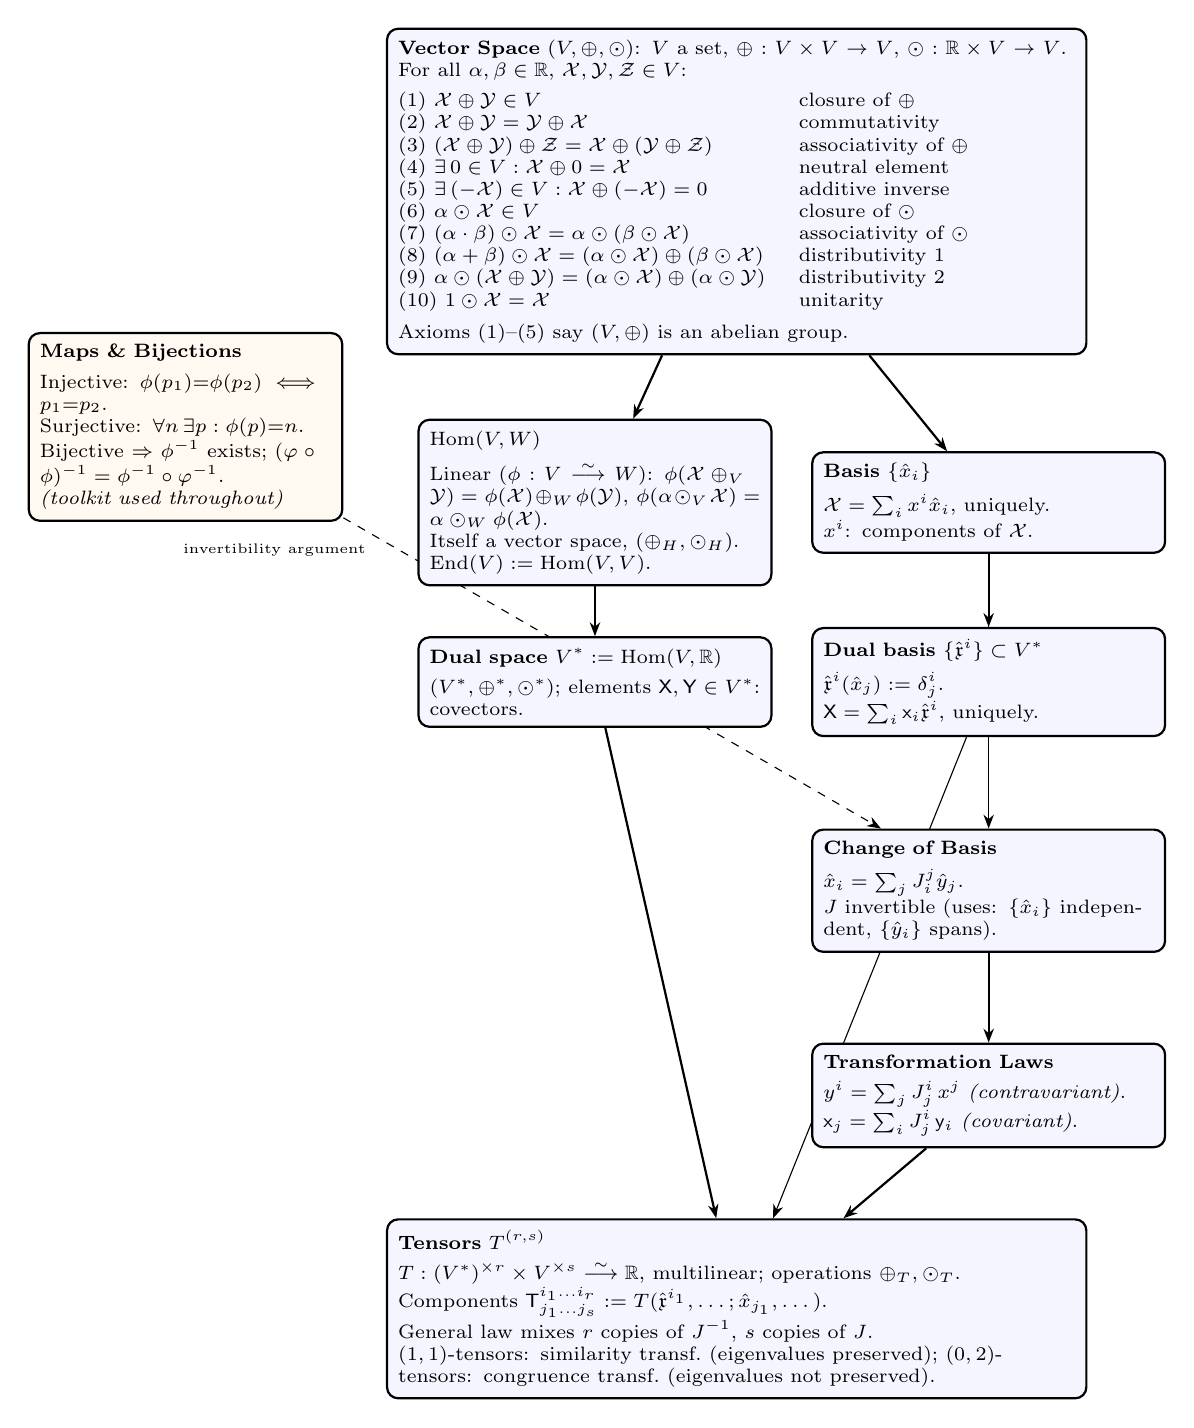
\begin{tikzpicture}[
  box/.style={draw, thick, rounded corners, fill=blue!4, align=left,
              text width=4.2cm, font=\scriptsize, inner sep=4pt},
  bigbox/.style={box, text width=8.6cm},
  aside/.style={box, text width=3.7cm, fill=orange!5},
  ->, >={Stealth[length=5pt]}, thick
]

% Root: full axiom list
\node[bigbox] (root) at (4.2,17.95) {%
  \textbf{Vector Space $\Vsp$}: $V$ a set, $\oplus:V\times V\to V$,
  $\odot:\mathbb R\times V\to V$. For all $\alpha,\beta\in\mathbb R$,
  $\mathcal X,\mathcal Y,\mathcal Z\in V$:\\[3pt]
  \begin{tabular}{@{}ll@{}}
  (1) $\mathcal X\oplus\mathcal Y\in V$ & closure of $\oplus$\\
  (2) $\mathcal X\oplus\mathcal Y=\mathcal Y\oplus\mathcal X$ & commutativity\\
  (3) $(\mathcal X\oplus\mathcal Y)\oplus\mathcal Z=\mathcal X\oplus(\mathcal Y\oplus\mathcal Z)$ & associativity of $\oplus$\\
  (4) $\exists\,0\in V:\mathcal X\oplus 0=\mathcal X$ & neutral element\\
  (5) $\exists\,(-\mathcal X)\in V:\mathcal X\oplus(-\mathcal X)=0$ & additive inverse\\
  (6) $\alpha\odot\mathcal X\in V$ & closure of $\odot$\\
  (7) $(\alpha\cdot\beta)\odot\mathcal X=\alpha\odot(\beta\odot\mathcal X)$ & associativity of $\odot$\\
  (8) $(\alpha+\beta)\odot\mathcal X=(\alpha\odot\mathcal X)\oplus(\beta\odot\mathcal X)$ & distributivity 1\\
  (9) $\alpha\odot(\mathcal X\oplus\mathcal Y)=(\alpha\odot\mathcal X)\oplus(\alpha\odot\mathcal Y)$ & distributivity 2\\
  (10) $1\odot\mathcal X=\mathcal X$ & unitarity
  \end{tabular}\\[3pt]
  Axioms (1)--(5) say $(V,\oplus)$ is an abelian group.
};

% Aside, top-left: Maps & Bijections (toolkit, not built from the root)
\node[aside] (bij) at (-2.8,14.96) {%
  \textbf{Maps \& Bijections}\\[3pt]
  Injective: $\phi(p_1){=}\phi(p_2)\!\iff\! p_1{=}p_2$.\\
  Surjective: $\forall n\,\exists p:\phi(p){=}n$.\\
  Bijective $\Rightarrow$ $\phi^{-1}$ exists;
  $(\varphi\circ\phi)^{-1}=\phi^{-1}\circ\varphi^{-1}$.\\
  \textit{(toolkit used throughout)}
};

% Level 1
\node[box] (hom) at (2.4,14.0) {%
  \textbf{$\mathrm{Hom}(V,W)$}\\[3pt]
  Linear ($\phi:V\linto W$): $\phi(\mathcal X\oplus_V\mathcal Y)=\phi(\mathcal X)\oplus_W\phi(\mathcal Y)$,
  $\phi(\alpha\odot_V\mathcal X)=\alpha\odot_W\phi(\mathcal X)$.\\
  Itself a vector space, $(\oplus_H,\odot_H)$.\\
  $\mathrm{End}(V):=\mathrm{Hom}(V,V)$.
};

\node[box] (basis) at (7.4,14.0) {%
  \textbf{Basis} $\{\hat x_i\}$\\[3pt]
  $\mathcal X=\sum_i x^i\hat x_i$, uniquely.\\
  $x^i$: components of $\mathcal X$.
};

% Level 2
\node[box] (dual) at (2.4,11.72) {%
  \textbf{Dual space} $\dual:=\mathrm{Hom}(V,\mathbb R)$\\[3pt]
  $(\dual,\oplus^*,\odot^*)$; elements $\mathsf X,\mathsf Y\in\dual$: covectors.
};

\node[box] (dbasis) at (7.4,11.72) {%
  \textbf{Dual basis} $\{\hat{\mathfrak x}^i\}\subset\dual$\\[3pt]
  $\hat{\mathfrak x}^i(\hat x_j):=\delta^i_j$.\\
  $\mathsf X=\sum_i\mathsf x_i\hat{\mathfrak x}^i$, uniquely.
};

% Level 3
\node[box] (cob) at (7.4,9.07) {%
  \textbf{Change of Basis}\\[3pt]
  $\hat x_i=\sum_j J_i^j\hat y_j$.\\
  $J$ invertible (uses: $\{\hat x_i\}$ independent, $\{\hat y_i\}$ spans).
};

% Level 4
\node[box] (tlaw) at (7.4,6.47) {%
  \textbf{Transformation Laws}\\[3pt]
  $y^i=\sum_j J_j^i\,x^j$ \emph{(contravariant)}.\\
  $\mathsf x_j=\sum_i J_j^i\,\mathsf y_i$ \emph{(covariant)}.
};

% Level 5
\node[bigbox] (tensor) at (4.2,3.76) {%
  \textbf{Tensors} $T^{(r,s)}$\\[3pt]
  $T:(\dual)^{\times r}\times V^{\times s}\linto\mathbb R$, multilinear; operations $\oplus_T,\odot_T$.\\
  Components $\mathsf T^{i_1\dots i_r}_{j_1\dots j_s}
  :=T(\hat{\mathfrak x}^{i_1},\dots;\hat x_{j_1},\dots)$.\\
  General law mixes $r$ copies of $J^{-1}$, $s$ copies of $J$.\\
  $(1,1)$-tensors: similarity transf.\ (eigenvalues preserved);
  $(0,2)$-tensors: congruence transf.\ (eigenvalues not preserved).
};

% Edges that cross no box: drawn on top, as usual
\draw (root) -- (hom);
\draw (root) -- (basis);
\draw (hom) -- (dual);
\draw (basis) -- (dbasis);
\draw (dual) -- (tensor);
\draw (cob) -- (tlaw);
\draw (tlaw) -- (tensor);

% Edges that cross exactly one box: drawn behind it (background layer)
\begin{pgfonlayer}{background}
  % basis -> cob passes directly behind dbasis (same column)
  \draw (basis) -- (cob);
  % dbasis -> tensor cuts diagonally behind cob
  \draw (dbasis) -- (tensor);
  % dashed "tool used in" edge cuts diagonally behind Dual space;
  % label is placed on the segment before the crossing
  \draw[dashed] (bij) -- (cob)
    node[pos=0.05, below left, yshift=-2pt, font=\tiny, fill=white, inner sep=1.5pt] {invertibility argument};
\end{pgfonlayer}

\end{tikzpicture}%
}
\end{center}

\end{document}
